\documentclass[autodetect-engine,dvipdfmx-if-dvi,ja=standard,b5paper,10.5pt,twoside,openany,layout=v2]{bxjsbook}

\newcommand{\stypath}{./sty}
\newcommand{\articlepath}{./articles}
\newcommand{\assetspath}{./assets}

\newcommand{\lrfasset}{\assetspath/lrf141asset}
\newcommand{\chikuwaitasset}{\assetspath/chikuwa_ITasset/gray}
\newcommand{\strvertasset}{\assetspath/strvertasset}
\newcommand{\haibaraaaaaaaaset}{\assetpath/haibaraaaaaaaaset}
\newcommand{\yuhiasset}{\assetpath/yuhiasset}
\newcommand{\materialofmouseasset}{\assetpath/materialofmouseasset}
\newcommand{\takuzoo3868}{\assetpath/takuzoo3868asset}

\usepackage{\stypath/localst17}
\usepackage{\stypath/mymintedsetting}

\usepackage{lipsum}
\usepackage{layout}

%keisuke495500
\usepackage{caption}

%Takuzoo3868
\usepackage{dirtree}

%Jumpaku
\usepackage{pxrubrica}
\usepackage{hyperref}
\usepackage{pxjahyper}
\usepackage{comment}
\usepackage{verbatim}

%materialofmouse
\usepackage{siunitx}

\usepackage{amsmath}
\usepackage{graphicx}

\title{情報ボーイズの寄稿ノート}
\author{うっひょい \and ちくうぇいと \and あわあわ \and けんつ \and さわだ \and Jumpaku \and あるねこ}

\date{}

\begin{document}
\frontmatter
\maketitle
\begin{myintroduce}{\chikuwaitasset/icon.jpg}{ちくうぇいと @chikuwa\_IT}
  RubyでイケイケWEBエンジニアになるつもりだったのに, 気がついたらmrubyをOSの下に組み込んだりして完全にシステムプログラミング沼に落ちてしまいました.\\
  どうしてこうなった.
\end{myintroduce}
\begin{myintroduce}{\lrfasset/icon_gray.jpg}{けんつ @lrf141}
  カーネルからWebまで色々やってます.\\
  インフラとScalaとJavaが大好物です.
\end{myintroduce}


\chapter{はじめに}
\addtolength{\oddsidemargin}{10pt}
\addtolength{\evensidemargin}{-10pt}
%\addtolength{\textwidth}{-14pt}
LOCALがくせーぶの紹介とかなんか.部長!お願いしますよ! by さわだ


\tableofcontents
\mainmatter
%\addtolength{\oddsidemargin}{-20pt}
%\addtolength{\evensidemargin}{18pt}

\chapterauthor{chikuwait(ちくうぇいと)}
\chapter{超入門 仮想化技術}
\section{はじめに}
近年, コンテナ型仮想化の普及もあり仮想化技術という存在を様々な場面でよく聞くようになりました. しかし, コンテナ型仮想化技術以外の他の仮想化技術というのは中々個人で扱うような技術・ソフトウェアではないこともあり, あまり知られていないことが多かったりします. また, コンテナ型仮想化技術も便利で環境構築が魔法のようなすごい存在といった漠然とした解釈の人もきっと多いはずです. そこでこの章では, 各種仮想化技術の仕組みや特徴について触れながらふわっと仮想化技術について紹介します.

\section{仮想化技術とは}
仮想化技術にはいくつか種類がありますが, この章では計算機資源を抽象化してOSなどに見せるプラットフォーム仮想化のことを指します. 仮想化することで複数の計算機資源を単一に見せたり, 単一の計算機資源を複数に見せることができます. そしてプラットフォーム仮想化を支えるための技術としてシステム仮想機械(VM, Virtual Machine)と呼ばれる計算機資源をエミュレートするソフトウェアが存在します. 仮想機械の実装は仮想マシンモニタ(VMM, Virtual Machine Monitor)を始めとしていくつか存在します. 例えば仮想専用サーバ(VPS, Virtual Private Server)のようなサービスでは図2.1にように, 物理サーバ上に仮想化OSによって複数の仮想サーバに分割してユーザに各仮想サーバを提供しています.
\begin{figure}[htbp]
    \centering
    \includegraphics[width=50mm]{./assets/chikuwa_ITasset/vps.png}
    \caption{hogehoge}
    \label{fig:one}
\end{figure}

\section{VMMについて}
仮想化を実現するVMMにはハイパーバイザ型(Type1),ホスト型(Type2)の2つに分類されます.

\subsection{ハイパーバイザー型(Type1)}
ハイパーバイザ型(Type1)は, ハードウェアの上で直接動作します. この方式ではホストOSと呼ばれるような土台になるOSが存在しないため,仮想マシンによる遅延や速度低下を防ぐことができます. そしてベアメタルハイパーバイザでは実装手法でもモノリシックカーネル型とマイクロカーネル型の2つに分類することができるほか, 仮想化のアプローチで完全仮想化と準仮想化に分類することができます.
\subsubsection{モノリシックカーネル型}
主にVMware ESX/ESXiなどで採用されている方式で, モノリシックという英語で「1枚岩」という意味の通り、VMMの中にデバイスドライバが含まれています. VMMがストレージをはじめ,ネットワークや入力デバイスといったハードウェアへのアクセスをすべてを処理します. この方法の利点はVMMとデバイスドライバが密接に連携するため,オーバーヘッドが少なく効率的です. しかしながら, VMMの中にデバイスドライバが存在しているため,ハイパーバイザ層でデバイスドライバを用意する必要があります. そのため, ハードウェアのサポートがマイクロカーネル型と比較して少なく, 使用するハードウェアに制限がかかってしまう場合があります. また, デバイスドライバをVMMに直接組み込むため, バグや脆弱性はVMM全体に広がってしまいます.
\begin{figure}[htbp]
    \centering
    \includegraphics[width=50mm]{./assets/chikuwa_ITasset/monolithic.png}
    \caption{モノリシックカーネル型ベアメタルハイパーバイザ}
    \label{fig:one}
\end{figure}
\begin{figure}[htbp]
    \centering
    \includegraphics[width=50mm]{./assets/chikuwa_ITasset/monolithic.png}
    \caption{モノリシックカーネル型のハードウェアアクセス}
    \label{fig:two}
\end{figure}
\subsubsection{マイクロカーネル型}
主にXenやHyper-Vで採用されている方式で, ハイパーバイザを管理する仮想マシンと管理OSを用意します. この管理OSはLinuxはWindows Serverなど汎用OSを使用します. また, 管理OSはXenではドメイン0, Hyper-Vでは親パーティションと呼ばれています. この方式では, デバイスドライバはVMMではなく, VMM上の仮想マシンとして動作している管理OSのデバイスドライバを使用します. 仮想マシンからハードウェアにアクセスする時はゲストOSから仮想デバイスのインターフェースを経由してVMMから管理OSに渡されます. そして管理OSのデバイスドライバからハードウェアにアクセスします.この方法は, 汎用OSのデバイスドライバを使用することで, モノリシックカーネル型に比べてハードウェアのサポートが多く, ハードウェアの対応が柔軟であるという利点があります. 例えば, Hyper-VならWindows用のデバイスドライバを使用することができます. しかしながら, ハードウェアにアクセスする際にVMMから管理OSを経由するため, モノリシックカーネル型よりも性能が低下してしまいがちであり, 管理用の汎用OSがクラッシュした場合全てのVMがクラッシュしてしまうといった欠点が存在します.
\begin{figure}[htbp]
    \centering
    \includegraphics[width=50mm]{./assets/chikuwa_ITasset/monolithic.png}
    \caption{マイクロカーネル型ベアメタルハイパーバイザ}
    \label{fig:one}
\end{figure}
\begin{figure}[htbp]
    \centering
    \includegraphics[width=50mm]{./assets/chikuwa_ITasset/monolithic.png}
    \caption{マイクロカーネル型のハードウェアアクセス}
    \label{fig:two}
\end{figure}

\subsubsection{完全仮想化}
完全仮想化方式のVMMでは, ハードウェアの挙動をすべてエミュレートします. そのため, 何も変更も加えていないそのままのホストOSを動かすことができます. 1960年代にIBMが「トラップアンドエミュレート」とよばれる方法で完全仮想化を実装しようとしました. この方法ではゲストOSが特権がない状態(Ring3)で実行させ, 特権(Ring0)が必要な命令を実行しようとすると失敗します. その際にVMMがその失敗をトラップして原因を確認してからその命令をエミュレートすることによってゲストOSの期待する結果を返すことができ, ゲストOSにRing0以外で実行されていることを気づかせないようにすることができます. しかしながら, この手法は古典的ですべてのアーキテクチャに適用できるわけではありませんでした. 特にx86プロセッサの場合, ユーザ権限で実行できるセンシティブ命令と呼ばれる計算機資源の構成などの依存している命令が存在しているため, 実装を難しくさせていました. そこで, 「バイナリトランスレーション」と呼ばれる新しい手法が使われるようになりました. この手法では, センシティブな命令以外の命令は直接CPUで実行し, センシティブな命令はVMMで実行前に動的に他の命令に置き換えられます.
\begin{figure}[htbp]
    \centering
    \includegraphics[width=50mm]{./assets/chikuwa_ITasset/monolithic.png}
    \caption{バイナリトランスレーション}
    \label{fig:one}
\end{figure}
\subsubsection{準仮想化}
\subsection{ホスト型(Type2)}


\chapterauthor{はいばら}
\chapter{後で変える}
\section{はじめに}
自宅サーバー,憧れますよね.そんな自宅サーバーをお手頃な価格で自作してしまいましょう.せっかくなのでモーターとタイヤをつけてしまいましょう.そうです,自走式WEBサーバーです.この章ではWiFiを扱うことのできるマイコン ESP-WROOM-02を用いた自走式WEBサーバーを作成します.
\footnote{本章に記載されたプログラム,回路図,その他工作物を参考にして製作した場合に生じた事故等について一切の責任を負いかねます.}
\subsection{ESP-WROOM-02とは}
ESP-WROOM-02は,上海の企業Espressif Systems のESP8266EXチップを搭載したWiFiモジュールです.いわゆる「技適」を取得しているため,日本国内で法的に安心して使えます.ardiono言語で開発できることに加え,おおよそ600円で購入できる手軽さが魅力です.
\footnote{ESP-WROOM-02の開発環境の構築方法については, ESP8266 Arduino Coreの公式ドキュメント(\url{https://arduino-esp8266.readthedocs.io/en/latest/})や僕のブログ(\url{https://haibara-works.hatenablog.com})の『ESP-WROOM-02を導入する』を参照してください.(ページ数の都合から割愛します)}

\subsection{ハードウェアの準備}
表\ref{buhin}に今回作る自走式WEBサーバーに必要な部品を示します.
\begin{table}[htb]
\centering
\caption{使うもの}
\begin{tabular}{|l|l|} \hline
部品 & 用途 \\ \hline \hline
ESP-WROOM-02 & ESP本体  \\ \hline
FT-232RQ & USBシリアル変換モジュール  \\ \hline
抵抗(10 K$\Omega$) & プルアップ・プルダウン用  \\ \hline
抵抗(470 K$\Omega$) & LEDの保護抵抗 \\ \hline
LED & パイロットランプ  \\ \hline
TA48033S & 電源レギュレータ(3.3 V) \\ \hline
コンデンサ(0.33 $\mu$F) & 電源用パスコン  \\ \hline
コンデンサ(33 $\mu$F) & 電源用パスコン  \\ \hline
TA7291P & モータードライバ \\ \hline
ダブルギヤボックス(左右独立4速タイプ) & タミヤのギヤボックス  \\ \hline
ブレッドボード & テスト用 \\ \hline
ジャンパ線 & テスト用 \\ \hline
\end{tabular}
\label{buhin}
\end{table}

\section{WEBサーバーとしての動作}

    \subsection{SPIFFSの利用}


\begin{minted}[frame=lines,framesep=2mm,baselinestretch=1.2,fontsize=\footnotesize,linenos,breaklines]{c}
#include <ESP8266WiFi.h>
#include <WiFiClient.h>
#include <ESP8266mDNS.h>
#include <ESP8266WebServer.h>
#include <ESP8266HTTPUpdateServer.h>
#include <FS.h>
#include "config.h"

const char* host = "esp8266fs";
ESP8266WebServer Server(80);      //80番ポートを使用

/**************************************************
  WEBサーバーに関する関数群
 **************************************************/
/**  Show URI args */
void showUriArgs() {
  Serial.printf("\n---URI args---\n");
  for (int i = 0; i < Server.args(); i++) {
    Serial.printf("%s: %s \n", Server.argName(i).c_str(), Server.arg(i).c_str());
  }
}

/**  ファイルの拡張子を調べてMIMEタイプを返す関数 */
String getContentType(String filename) {
  if (Server.hasArg("download")) return "application/octet-stream";
  else if (filename.endsWith(".htm")) return "text/html";
  else if (filename.endsWith(".html")) return "text/html";
  else if (filename.endsWith(".css")) return "text/css";
  else if (filename.endsWith(".js")) return "application/javascript";
  else if (filename.endsWith(".png")) return "image/png";
  else if (filename.endsWith(".gif")) return "image/gif";
  else if (filename.endsWith(".jpg")) return "image/jpeg";
  else if (filename.endsWith(".ico")) return "image/x-icon";
  else if (filename.endsWith(".xml")) return "text/xml";
  else if (filename.endsWith(".pdf")) return "application/x-pdf";
  else if (filename.endsWith(".zip")) return "application/x-zip";
  else if (filename.endsWith(".gz")) return "application/x-gzip";
  else return "text/plain";
}

/**  指定されたパスのファイルをクライアントに送信 */
void handleSendRes(void) {
  showUriArgs();
  String path = Server.uri();

  if (path.equals("/motor.html")) {
    motor._mode = Open;
    if (Server.arg("motorMode").equals("forw")) {
      motor._mode = Forw;
    } else if (Server.arg("motorMode").equals("back")) {
      motor._mode = Back;
    } else if (Server.arg("motorMode").equals("right")) {
      motor._mode = Right;
    } else if (Server.arg("motorMode").equals("left")) {
      motor._mode = Left;
    }
    motor.val = atoi(Server.arg("motorVal").c_str());
  }

  Serial.println("");
  Serial.println("[handleSendRes]: trying to read " + path);

  if (path.endsWith("/")) path += "index.html";

  String contentType = getContentType(path);

  if (SPIFFS.exists(path)) {
    Serial.println("[handleSendRes]: sending " + path);
    File file = SPIFFS.open(path, "r");
    Server.streamFile(file, contentType);
    file.close();
    Serial.println("[handleSendRes]: sent " + path);
  } else {
    Serial.println("[handleSendRes]: 404 not found");
    Server.send (404, "text/plain", "ESP: 404 not found");
  }
}

/**  settings */
void setup() {
  motor._mode = Open;
  motor.val = 0;

  Serial.begin(74880);

  pinMode(Pilot, OUTPUT);
  digitalWrite(Pilot, HIGH);

  motorSetup(M1_l, M1_r, M2_l, M2_r);

  WiFi.mode(WIFI_STA);
  WiFi.begin(ssid, pass);
  delay(100);

  Serial.println("");

  while (WiFi.status() != WL_CONNECTED) {
    delay(500);
    digitalWrite(Pilot, !digitalRead(Pilot));
    Serial.print(".");
  }
  digitalWrite(Pilot, HIGH);

  Serial.println("");
  Serial.print("Connected to ");
  Serial.println(ssid);
  Serial.print("IP address: ");
  Serial.println(WiFi.localIP());
  MDNS.begin(host);

  SPIFFS.begin();
  {
    Dir dir = SPIFFS.openDir("/");
    while (dir.next()) {
      String fileName = dir.fileName();
      size_t fileSize = dir.fileSize();
      Serial.printf("FS File: %s, size: %s\n", fileName.c_str(), formatBytes(fileSize).c_str());
    }
    Serial.printf("\n");
  }

  //  ウェブサーバの設定
  Server.on("/list", HTTP_GET, handleFileList);
  Server.on("/edit", HTTP_GET, []() {
    if (!handleFileRead("/edit.htm")) {
      Server.send(404, "text/plain", "FileNotFound");
    }
  });
  Server.on("/edit", HTTP_PUT, handleFileCreate);
  Server.on("/edit", HTTP_DELETE, handleFileDelete);
  Server.on("/edit", HTTP_POST, []() {
    Server.send(200, "text/plain", "");
  }, handleFileUpload); 
  Server.on("/all", HTTP_GET, []() {
    String json = "{";
    json += "\"heap\":" + String(ESP.getFreeHeap());
    json += ", \"analog\":" + String(analogRead(A0));
    json += ", \"gpio\":" + String((uint32_t)(((GPI | GPO) & 0xFFFF) | ((GP16I & 0x01) << 16)));
    json += "}";
    Server.send(200, "text/json", json);
    json = String();
  });
  Server.onNotFound(handleSendRes);  ////called when handler is not assigned
  
  Server.begin();
}

/**  main loop */
void loop() {
  Server.handleClient();
  MDNS.update();

  switch (motor._mode) {
    case Forw:
      goForward(motor.val);
      break;
    case Back:
      goBack(motor.val);
      break;
    case Right:
      turnRight(motor.val);
      break;
    case Left:
      turnLeft(motor.val);
      break;
    case Open:
    default:
      stopMotor();
  }
}
\end{minted}


\section{ラジコンとしての動作}
%    \subsubsection{}

\begin{minted}[frame=lines,framesep=2mm,baselinestretch=1.2,fontsize=\footnotesize,linenos,breaklines]{c}
enum { M1_l = 4, M1_r = 5, M2_l = 12, M2_r = 13, Pilot = 16,
       Stop, Open, Forw, Back, Right, Left };

typedef struct {
  int _mode;
  int val;
} motor_T;
motor_T motor;

/**************************************************
  モーター制御に関する関数群
 **************************************************/
/**  左右2つのモーターに接続されるピンを初期化 */
void motorSetup(const int m1_l, const int m1_r, const int m2_l, const int m2_r) {
  pinMode(m1_l, OUTPUT);
  pinMode(m1_r, OUTPUT);
  pinMode(m2_l, OUTPUT);
  pinMode(m2_r, OUTPUT);

  digitalWrite(m1_l, LOW);
  digitalWrite(m1_r, LOW);
  digitalWrite(m2_l, LOW);
  digitalWrite(m2_r, LOW);

  analogWriteFreq(5);
}

/**  モーターをPWM制御する関数 */
void motorDrive(int16_t pwmVal, const int m_l, const int m_r) {
  pwmVal = constrain(pwmVal, -1024, 1024);

  if (pwmVal >= 0) {
    analogWrite(m_l, pwmVal);
    digitalWrite(m_r, LOW);
  } else {
    pwmVal = abs(pwmVal);

    digitalWrite(m_l, LOW);
    analogWrite(m_r, pwmVal);
  }
}

/**  stop */
void stopMotor() {
  digitalWrite(M1_l, LOW);
  digitalWrite(M1_r, LOW);
  digitalWrite(M2_l, LOW);
  digitalWrite(M2_r, LOW);
}

/**  前進 */
void goForward(int16_t velocity) {
  motorDrive(velocity, M1_l, M1_r);
  motorDrive(velocity, M2_l, M2_r);
}

/**  後進 */
void goBack(int16_t velocity) {
  motorDrive(-velocity, M1_l, M1_r);
  motorDrive(-velocity, M2_l, M2_r);
}

/**  右旋回 */
void turnRight(int16_t velocity) {
  motorDrive(velocity, M1_l, M1_r);
  motorDrive(-velocity, M2_l, M2_r);
}

/**  右旋回 */
void turnLeft(int16_t velocity) {
  motorDrive(-velocity, M1_l, M1_r);
  motorDrive(velocity, M2_l, M2_r);
}
\end{minted}

\section{おわりに}
ESP-WROOM-02を使って自走式WWEBサーバーを作成することができた.今後の課題として,websocketを用いたリアルタイム性の高い操作を実現したい.また,今回の


\chapterauthor{けんつ}
\chapter{入門Linux Kernel}
\section{はじめに}

最近の開発、主にその開発環境やインフラレイヤーにおいて無くてはならないものとしてDockerが挙げられる。そして、Dockerを使ってWebサービスのインフラ等を構築する場合よく利用するのはdocker-composeだろう。
この章ではDockerの基本的な部分から紹介し、docker-composeの裏側を解説したあとにDocker Remote APIを使って自分でコンテナを制御するということについて紹介する。


\section{Dockerとは}

Dockerそのものに関しては公式ドキュメントよりもさくらインターネットさんの「さくらのナレッジ Docker入門(第一回)~Dockerとは何か、何が良いのか~」で簡単に紹介されていたのでそちらを引用する。
Dockerとはその記事で次のように紹介されている。\cite{sakura}

\begin{quote}
Dockerは、インフラ関係やDevOps界隈で注目されている技術の一つで、Docker社が開発している、コンテナ型の仮想環境を作成、配布、実行するためのプラットフォームです。
(https://www.docker.com/what-docker)

Dockerは、Linuxのコンテナ技術を使ったもので、よく仮想マシンと比較されます。VirtualBoxなどの仮想マシンでは、ホストマシン上でハイパーバイザを利用しゲストOSを動かし、その上でミドルウェアなどを動かします。それに対し、コンテナはホストマシンのカーネルを利用し、プロセスやユーザなどを隔離することで、あたかも別のマシンが動いているかのように動かすことができます。そのため、軽量で高速に起動、停止などが可能です。
\end{quote}

これが全てとなる。Dockerコンテナを利用することで特にWebサービス開発の開発環境において共通のインフラをチーム全員で共有することができるなどの様々なメリットがある。


\subsection{Dockerのアーキテクチャ}
Dockerとはコンテナの色々に関わるプラットフォームを指しているが実際にコンテナを利用する場合にはdockerコマンドを通して使う場合が多い。
dockerコマンドは何をしているかというと、docker remote apiを呼び出している。このdocker remote apiなるものは、Dockerのアーキテクチャに深く関係している。


Dockerのアーキテクチャはクライアント・サーバアーキテクチャとなっておりdockerコマンドはただのCLIツールである。
そのただのCLIツールが何をしているかというとdocker daemonが提供しているREST APIライクなDocker Remote APIをコールしているに過ぎない。


Docker Remote APIはデフォルトでunixドメインソケットを用いることで利用できるようになっている。自身で設定することでtcpによるリクエストを許可することも出来る。これ移行の章ではそれを有効にしている前提で話を進めていく。

\section{Docker Composeとは}

Docker-Composeとは、前述のDockerコンテナを複数利用する場合にそれらをまとめて管理するためのツールである。
Dockerコマンドだけでは何が問題かというと、例えばweb開発においてインフラをDockerコンテナで用意するならばNginxのコンテナにMySQLのコンテナ、PHPやRailsが動作するコンテナなど複数のコンテナが必要になってくる。
これら全てをdocker runで呼び出すとシェルなどにまとめておく必要がある。そして利便性に欠ける。では、サービスに必要なコンテナ群を一箇所でまとめて管理してしまいたい。そういう場合にdocker-composeを利用するのは非常に有効な手段となる。


そして、Docker ComposeはDocker Remote APIを通してdocker-compose.ymlに記載されているコンテナ群を管理している。
この点がこれ移行の説明で非常に重要になっていく。

\section{docker-composeを自作する}

ここまで紹介した情報を元にこの章の本題である、Dockerコンテナの制御を行う。制御といっても何をするかというとDocker Remote APIを使って超絶最高にシンプルなdocker-composeを作ってみる。Golangで。書いたことあまりないけど。


それではまず要件を以下に定義する。
\begin{itemize}
    \item ymlを解析して作成するコンテナやボリューム、ポートを設定できる
    \item コンテナを走らせる。
    \item コンテナを落とす。
    \item 起動しているコンテナのステータスを取る
\end{itemize}

\subsection{コマンドライン引数をパースする}

まずは、cliツールを作る上でコマンドライン引数をパースする必要がある。そこで import flag を使って簡易的にパースしていく。今回のcliツールではup,down,statusまでできれば十分なのでそれだけ定義する。

\begin{minted}[frame=lines,framesep=2mm,baselinestretch=1.2,fontsize=\footnotesize,linenos,breaklines]{go}
package main

import (
    "flag"
    "fmt"
)

func main() {
    flag.Parse()

    switch flag.Arg(0) {

    case "up":
        fmt.Println("up")
    case "down":
        fmt.Println("down")
    case "status":
        fmt.Println("status")
    default:
        fmt.Println("unknown")
    }
}
\end{minted}

\subsection{ymlをパースする}

次にそれなりに重要な機能であるymlのパースを行う。ただパーサーから書いている時間はなかったのでここでは gopkg.in/yaml.v2 というパッケージを使用する。

\begin{minted}[frame=lines,framesep=2mm,baselinestretch=1.2,fontsize=\footnotesize,linenos,breaklines]{go}
package main

import (
    "flag"
    "fmt"
    yaml "gopkg.in/yaml.v2"
    "io/ioutil"
)

type Services struct {
    Services []Docker `yaml:"services"`
}

type Docker struct {
    Name string     `yaml:"name"`
    Image string    `yaml:"image"`
    Command string  `yaml:"command"`
}

func main() {

    buf, err := ioutil.ReadFile("./lite-compose.yml")
    if err != nil {
        panic(err)
    }

    var parsed Services
    err = yaml.Unmarshal(buf, &parsed)
    if err != nil {
        panic(err)
    }

    fmt.Println(parsed)

    flag.Parse()
    switch flag.Arg(0) {

    case "up":
        fmt.Println("up")
    case "down":
        fmt.Println("down")
    case "status":
        fmt.Println("status")
    default:
        fmt.Println("unknown")
    }
}
\end{minted}

コード自体はこれでいいのだがひとつ問題がある。docker-composeのようなパターンのymlを今回使ったライブラリではパースできないことだ。
しかし、パーサーから探すのはめんどくさいので仕方なくymlの形式を以下のようにして lite-compose.yml とする。

\begin{minted}[frame=lines,framesep=2mm,baselinestretch=1.2,fontsize=\footnotesize,linenos,breaklines]{yaml}

services:
-
  name: ubuntu
  image: ubuntu
  command: 'echo "hello, world"'

\end{minted}

これを実行すると構造体として表示される。ただこれだけでは色々と不十分なのでエラーハンドリングを追加してファイルを分割してみた。

\begin{minted}[frame=lines,framesep=2mm,baselinestretch=1.2,fontsize=\footnotesize,linenos,breaklines]{go}
package main

import (
    "flag"
    "fmt"
    "gopkg.in/yaml.v2"
    "io/ioutil"
)

func main() {

    buf, err := ioutil.ReadFile("./lite-compose.yml")
    if err != nil {
        panic(err)
    }

    var parsed Services
    err = yaml.Unmarshal(buf, &parsed)
    if err != nil {
        panic(err)
    }

    if err := requireNotExist(); !parsed.validate() {
        panic(err)
    }

    flag.Parse()
    switch flag.Arg(0) {

    case "up":
        fmt.Println("up")
    case "down":
        fmt.Println("down")
    case "status":
        fmt.Println("status")
    default:
        fmt.Println("unknown")
    }
}
\end{minted}

\begin{minted}[frame=lines,framesep=2mm,baselinestretch=1.2,fontsize=\footnotesize,linenos,breaklines]{go}
package main

import "errors"

type Services struct {
    Services []Docker `yaml:"services"`
}

type Docker struct {
    Name string     `yaml:"name"`
    Image string    `yaml:"image"`
    Command string  `yaml:"command"`
}

func (services *Services) validate() bool {
    for _, docker := range services.Services {
        if docker.Image == "" || docker.Name == "" {
            return false
        }
    }
    return true
}


func requireNotExist() error {
    return errors.New("The syntax of yaml is incorrect")
}
\end{minted}

\section{コンテナを制御する}

ここまでやってきたら後はdocker remote apiを使ってdockerコンテナを立ち上げ落としてステータスを取れるようにする。
docker remote api自体はunixドメインソケットかtcpまたはhttpでリクエストを飛ばすことで利用することができる。ここではそれらを順を追って説明していく。
本来はそれらリクエスト部分を自作するつもりであったが今回は golang でdocker remote apiを利用できるライブラリのgithub.com/docker/dockerを使用する。


実際にdocker remote apiを使ったコンテナ制御は以下のようになる。
\begin{minted}[frame=lines,framesep=2mm,baselinestretch=1.2,fontsize=\footnotesize,linenos,breaklines]{go}
package main

import (
    "context"
    "fmt"
    "github.com/docker/docker/api/types"
    "github.com/docker/docker/api/types/container"
    "github.com/docker/docker/api/types/network"
    "github.com/docker/docker/client"
    "os"
    "strings"
    "time"
)

func createContainer(services Services) {
    ctx := context.Background()
    cli, err := client.NewClientWithOpts(client.WithVersion("1.39"))
    if err != nil {
        panic(err)
    }

    p, _ := os.Getwd()
    split := strings.Split(p, "/")
    current := split[len(split)-1]

    for _, service := range services.Services {

        hostConfig := &container.HostConfig{}
        containerConfig := &container.Config{
            Image: service.Name,
            Tty: true,
            Cmd: strings.Split(service.Command, " "),
        }
        networkConfig := &network.NetworkingConfig{}

        resp, err := cli.ContainerCreate(ctx, containerConfig, hostConfig, networkConfig, current+"_"+service.Name)
        if err != nil {
            fmt.Println(err)
        } else {
            err := cli.ContainerStart(ctx, resp.ID, types.ContainerStartOptions{})
            if err != nil {
                fmt.Println(err)
            } else {
                fmt.Println(resp)
            }

        }
    }
}

func killContainer(services Services) {
    ctx := context.Background()
    cli, err := client.NewClientWithOpts(client.WithVersion("1.39"))
    if err != nil {
        panic(err)
    }

    p, _ := os.Getwd()
    split := strings.Split(p, "/")
    current := split[len(split)-1]

    timeout := 5 * time.Second

    for _, service := range services.Services {
        resp := cli.ContainerStop(ctx, current+"_"+service.Name, &timeout)
        fmt.Println(resp)
    }
}

func getDockerImageList() {

    ctx := context.Background()
    cli, err := client.NewClientWithOpts(client.WithVersion("1.39"))
    if err != nil {
        panic(err)
    }

   list, err := cli.ImageList(ctx, types.ImageListOptions{})
   if err != nil {
        panic(err)
   }

   for _, image := range list {
       fmt.Printf("RepoTags: %s, Labels: %s, Container: %d, Size: %d\n", image.RepoTags, image.Labels, image.Containers, image.Size)
   }

}


func getDockerPs() {
    ctx := context.Background()
    cli, err := client.NewClientWithOpts(client.WithVersion("1.39"))
    if err != nil {
        panic(err)
    }

    containers, err := cli.ContainerList(ctx, types.ContainerListOptions{
        All: true,
    })

    if err != nil {
        panic(err)
    }

    for _, container := range containers {
        fmt.Printf("ID: %s, Name: %sm Image: %s, Command: %s\n", container.ID, container.Names, container.Image, container.Command)
    }
}
\end{minted}

ここでは、ライブラリを使用してHostConfigなどを設定し、コンテナを作成した上で起動させるという一連の流れを行っている。
さらにportsやvolumesなど今回は導入しなかったが通常docker-compose.ymlで設定するようなパラメータ群を設定することもできるので興味があれば実際に試して欲しい。

\section{おわりに}

ここで紹介したように、dockerとはプラットフォームであり普段使うようなdockerコマンドは実際にはdocker remote apiを叩いているに過ぎない。また、docker-composeはそれらをまとめて管理しているがこれもまたdocker remote apiを叩いているだけである。
そのため、これらを応用すれば競技プログラミングやオンライン実行環境で実際にコードを動かす部分をユーザのアクションに併せて作成することができる。
是非そのようなサービスを開発する際にここに書いてある知識を応用して貰えると締め切りの前日からこのようなものを作り始めた甲斐があるというものである。


\begin{thebibliography}{10}
    \bibitem{sakura} Docker入門(第一回)~Dockerとは何か、何が良いのか~ | さくらのナレッジ https://knowledge.sakura.ad.jp/13265/
    \bibitem{unixdomain} tcp-hist.ps http://osnet.cs.binghamton.edu/publications/TR-20070820.pdf
\end{thebibliography}


\chapterauthor{さわだ}
\chapter{後で変える}
\section{はじめに}
皆さんはちょっとしたメモやプログラミングにどんなエディタを使いますか?Vim?それともEmacs?まぁ色々ありますよね.
人それぞれ好き嫌いがあると思います.僕はVimを自分好みに拡張するのが好きです\footnote{そこのEmacs教徒,石を投げないで!}.
でも,人には自作欲求があります.CPU,OS,言語,更に最近はキーボードなどが人気ですが,エディタも中々面白いですよ.
CUIは時代遅れなんてそんなの気にしちゃいけません.
ソースコードは\url{https://github.com/takuzoo3868/td}に置いてあります.

\section{準備}
テキストエディタと言いつつも初めから高機能なエディタを自作するのは至難の業です.
そこで,最低限ファイルを編集して保存できるようにする所から始めるといいかなと思います.
次にシンタックスハイライト対応や文字列検索機能などを考えていきましょう.
リポジトリにあるテキストエディタのファイル構造は以下ようになっています.

\begin{figure}[H]
    \dirtree{%
    .1 td/.
    .2 modules/ \dotfill  \begin{minipage}[t]{7cm}
                              拡張機能を追加していくディレクトリ{.}
    \end{minipage}.
    .3 syntax/ \dotfill  \begin{minipage}[t]{7cm}
                             シンタックスハイライト用の構造体を定義{.}
    \end{minipage}.
    .2 LICENSE.
    .2 Makefile.
    .2 README.md.
    .2 td.c \dotfill  \begin{minipage}[t]{7cm}
                              メインとなるソースコード{.}
    \end{minipage}.
    .2 td.h \dotfill  \begin{minipage}[t]{7cm}
                              定数定義や構造体を含むヘッダ{.}
    \end{minipage}.
    }
\end{figure}
外部ライブラリに依存しない事を目標としていますが,Cコンパイラと\mintinline{bash}{make}コマンドは準備する必要があります.
\mintinline{bash}{cc --version}や\mintinline{bash}{make -v}でインストールされているかどうか確認できます.
自身の環境にコンパイラがインストールされていなかった場合は,Google先生に聞いてみましょう.

\subsubsection{makeによるコンパイル}
解説のために本文中では\mintinline{bash}{hoge}と記載しますが,
好きな名前に置き換えて下さい.
\mintinline{bash}{cc hoge.c -o hoge}などと打ち込めばコンパイルできます.
しかし試行錯誤を繰り返すため,再コンパイルの度に同じ事をするのはあまりスマートではありません.
\mintinline{bash}{make}を用いることでプログラムコンパイルを少しだけ楽にしておきましょう.
\mintinline{bash}{Makefile}を作成し,以下の内容を記述しておきます.
\begin{minted}[frame=lines,framesep=2mm,baselinestretch=1.2,fontsize=\footnotesize,linenos,breaklines]{text}
hoge: hoge.c
$(CC) -o hoge hoge.c -Wall -W -pedantic -std=c99
\end{minted}
この辺については,準備段階なので詳細は省きます.とてもざっくりに言いますと,
諸々の構文をチェックして警告を表示してくれるようオプションを設定しています.これで準備は完了です.

\section{基本構成}
基本となる骨格はkiloというテキストエディタを参考にします\footnote{\url{https://github.com/antirez/kilo}}.
Salvatore Sanfilippo氏によって開発されたC言語製のエディタです.BSD 2-clauseにて公開されています.
紹介文に,
\begin{quote}
Kilo is a small text editor in less than 1K lines of code (counted with cloc).
\end{quote}
とあるように1000行程度なので目で追っていくもの問題ないでしょう.ちょっと厳しいという方は\mintinline{c}{int main()}だけでも目を通す事をお勧めします.
\inputminted[frame=lines,framesep=2mm,baselinestretch=1.2,fontsize=\footnotesize,linenos,breaklines]{c}{\takuzooasset/main.c}
処理の流れはコメントの通り,
\begin{enumerate}
\item 起動にあたりエディタの初期化
\item 引数にあるファイルの拡張子に対応したシンタックスハイライトを適用
\item ファイルをメモリ上へ展開
\item エスケープシーケンスを利用してターミナルをRaw modeへ変更
\item ループ処理
\end{enumerate}
となります.ループでは画面反映とキー入力待ちを行っています.本書では入門編という事でRaw modeの作成を一緒に頑張っていきましょう.

\section{Build your own Editor!!!}
\subsection{Step.1 Raw modeの作成}
ここまでで自作エディタのための開発環境構築は終わっているものとします.
プログラムを書くために,どのエディタを使うかはご自身の信条に従って下さい.
それでは最初の一歩です.以下のコードを書いてみましょう.
\inputminted[frame=lines,framesep=2mm,baselinestretch=1.2,fontsize=\footnotesize,linenos,breaklines]{c}{\takuzooasset/step1_1.c}
\mintinline{c}{unistd.h}から\mintinline{c}{read()}と\mintinline{c}{STDIN_FILENO}を呼び出しています.
\mintinline{c}{read()}は標準入力から1byteを変数\mintinline{c}{c}に読み込んで,読み取るバイトデータがなくなるまで繰り返すようにしてあります.
コンパイルしプログラムを実行すると,端末は標準入力に接続され,キーボードの入力が変数\mintinline{c}{c}に読み込まれます
\footnote{プログラムを終了する場合はCtrl-Dで\mintinline{c}{read()}へ最後へ到達したことを知らせるか,Ctrl-Cでプロセスを終了します.}.
しかし,多くの場合端末は\mintinline{bash}{canonical mode}で起動\footnote{\mintinline{bash}{cooked mode}とも言います}するので,
\mintinline{bash}{raw mode}へ切り替える必要があります.
\mintinline{bash}{canonical mode}はEnterキーを押す事でキーボード入力がプログラムへ渡されます.
テキストエディタの場合は,複雑なインターフェースに加え,キーを押したあとにすぐ処理をしたいので\mintinline{bash}{canonical mode}が適しているとは言えません.
というこで,端末を\mintinline{bash}{raw mode}へ変更しますが,端末内部のフラグをoffにする必要があるので徐々に解説します.

\subsubsection{\mintinline{bash}{ECHO}をoffにする}
端末の\mintinline{bash}{ECHO}機能は入力したキー情報が端末画面に表示され,内容を確認できる優れた機能です.
しかし,レンダリングにおいて\mintinline{bash}{raw mode}では適していないのも事実です.よってoffにしちゃいましょう
\footnote{\mintinline{bash}{sudo}でパスワードを入力するイメージに近いです.}.
\inputminted[frame=lines,framesep=2mm,baselinestretch=1.2,fontsize=\footnotesize,linenos,breaklines]{c}{\takuzooasset/step1_2.c}
手順としては\mintinline{c}{tcgetattr()}を使用して現在の属性を\mintinline{c}{termios}構造体へ読み込み,構造体の変更,
変更された構造体を\mintinline{c}{tcgetattr()}へ渡し,新しい端末属性を書き込むという事をしています.
\mintinline{c}{TCSAFLUSH}は変更をいつ適用するかを指定する引数です.
\mintinline{c}{c_lflag}はローカル用のフラグです.雑多なフラグを管理するためにあります\footnote{macOSの\mintinline{c}{termios.h}には"Local" flags - dumping ground for other stateと書いてあります.}.
そのほか\mintinline{bash}{raw mode}の有効化に関連して変更するフラグは,\mintinline{c}{c_iflag}の入力フラグ,\mintinline{c}{c_oflag}の出力フラグ,\mintinline{c}{c_cflag}の制御フラグです.

次に必要な要素として,プログラムの終了時は端末の元の属性を復元してあげる必要があります.
\mintinline{c}{atexit()}はプログラム終了時に自動的に\mintinline{c}{disableRawMode}を呼び出すために使用します.
端末の元の属性は,\mintinline{c}{orig_termios}構造体に保存しておきます.

\subsubsection{\mintinline{bash}{canonical}のoffとキー入力}
\mintinline{bash}{canonical mode}をoffにするフラグは\mintinline{c}{termios.h}にある\mintinline{c}{ICANON}です.
offにすることで行単位ではなくバイト単位で入力を読み取ることになります.
先程のプログラムの15行目を\mintinline{c}{raw.c_lflag &= ~(ECHO | ICANON);}へ変更し実行してみましょう.
終了時はqキーを押せば大丈夫です.これで\mintinline{bash}{raw mode}へ移行できるようになりました.
それでは入力の様子を知るべく,\mintinline{c}{read()}で読み込んだ各バイトを出力してみましょう.
\inputminted[frame=lines,framesep=2mm,baselinestretch=1.2,fontsize=\footnotesize,linenos,breaklines]{c}{\takuzooasset/step1_3.c}
実行してみると画面にキー入力の結果,どのようにバイト変換されているか表示されるはずです.
\mintinline{c}{iscntrl()}は入力が制御文字かどうか調べてくれます.制御文字とは,画面上に表示できないASCIIコード\footnote{http://www.asciitable.com/}の事を指します.

\subsubsection{出力処理のoffとエラー処理}
ここまで完了したらあとはテキストエディタ用に雑多な処理を記述するだけです.コードは少し長くなります.
\inputminted[frame=lines,framesep=2mm,baselinestretch=1.2,fontsize=\footnotesize,linenos,breaklines]{c}{\takuzooasset/step1_4.c}
どんな処理を追加したかというと,Ctrl-C,Ctrl-Z,Ctrl-S,Ctrl-Q,Ctrl-Vを無効化し,Ctrl-Mを\mintinline{bash}{carriage return}へ修正.
さらに\mintinline{c}{termios.h}に記載されているいくつかのフラグを無効化しています.あとはエラー処理と\mintinline{c}{read()}のタイムアウトなんかも設定しています.
なんか説明が雑だなと思ったあなたごめんなさい\footnote{実装内容やプログラムの詳細については次の執筆機会か,あるいは自分のブログに書きます. http://takuzoo3868.hatenablog.com/}.ページの都合です\verb#(´;ω;`)#

\section{おわりに}
今回は入門編という事で\mintinline{bash}{raw mode}の実装のみに絞りました.
今後プログラムとして実装するステップを述べておくと,
\begin{enumerate}
\item Raw modeにおける入出力処理
\item テキストビューワーの作成
\item 編集処理
\item 文字列検索機能
\item シンタックスハイライト
\end{enumerate}
となります.自分のリポジトリではこれらステップを全て実装済みなのでコードを確認していただけると良いかなと思います.
勿論GUIアプリケーションとして開発したい方もいるでしょう.自分も今実践中なのでもし興味ある方は連絡\footnote{https://takuzoo3868.github.io/}ください!
それでは,よい自作ライフを!!!

\chapterauthor{あわあわくん}
\chapter{後で変える}
\section{自己紹介}
こんにちは、あわあわくん()(@materialofmouse)です。
同人誌を書く話になったのでLEDでひたすら発電してみました。
この章ではLEDで発電という普通はやらないことをやっています。
それに検証性がないのでちゃんと書かれてません。おまけだとおもって読んでください。

\section{LEDで発電できるの?}
できます。
詳しい話はインターネットで出てきますので、興味があるかたはぜひ調べてみてください。


\section{実際に発電してみる}
LEDで発電できるのか、実際に試したいと思います。
ものが近くにある方はぜひやってみてください。
\begin{description}
  \item[場所]{近くの駐車場}
  \item[時間]{14:10}
  \item[光源]{太陽光}
  \item[照度]{$160,000\si\lux$}
  \item[天気]{雲ひとつない晴れ}
\end{description}


\subsection{LED1個}
まず、LEDを1個。アノード側にテスターのプラス、カソード側にテスターのマイナスを接続します。
図\ref{fig:led1}の状態でLEDを太陽の方へ向けてみます。そこで発生した電流と電圧の値を取っていきます。
手元の環境では、普通の白色LEDから約10$\mu\si\ampere$,約1.2$\si\volt$発生しました。

\begin{figure}[htbp]
    \centering
    \includegraphics[width=60mm]{./assets/mouse/gray/a.JPG}
    \caption{LED1個で電流と電圧を測定している様子}
    \label{fig:led1}
\end{figure}

\subsection{直列と並列どちらが良いのか考える}
先ほどはLED1個で発電してみましたが、次は複数接続してみたいと思います。
複数接続にあたり、直列接続と並列接続のどちらが発電に適しているのかを実験してみました。

LED2個を直列に接続し、その両端をテスターで見ていきます。
図\ref{fig:led2}に測定の様子を示します.
そこに光を与えたところ、約100$\mu\si\ampere$,約2.5$\si\volt$発生しました。
この結果から、LED1個の時と比べ、電流、電圧ともに2倍になっていることがわかります。

\begin{figure}[htbp]
    \centering
    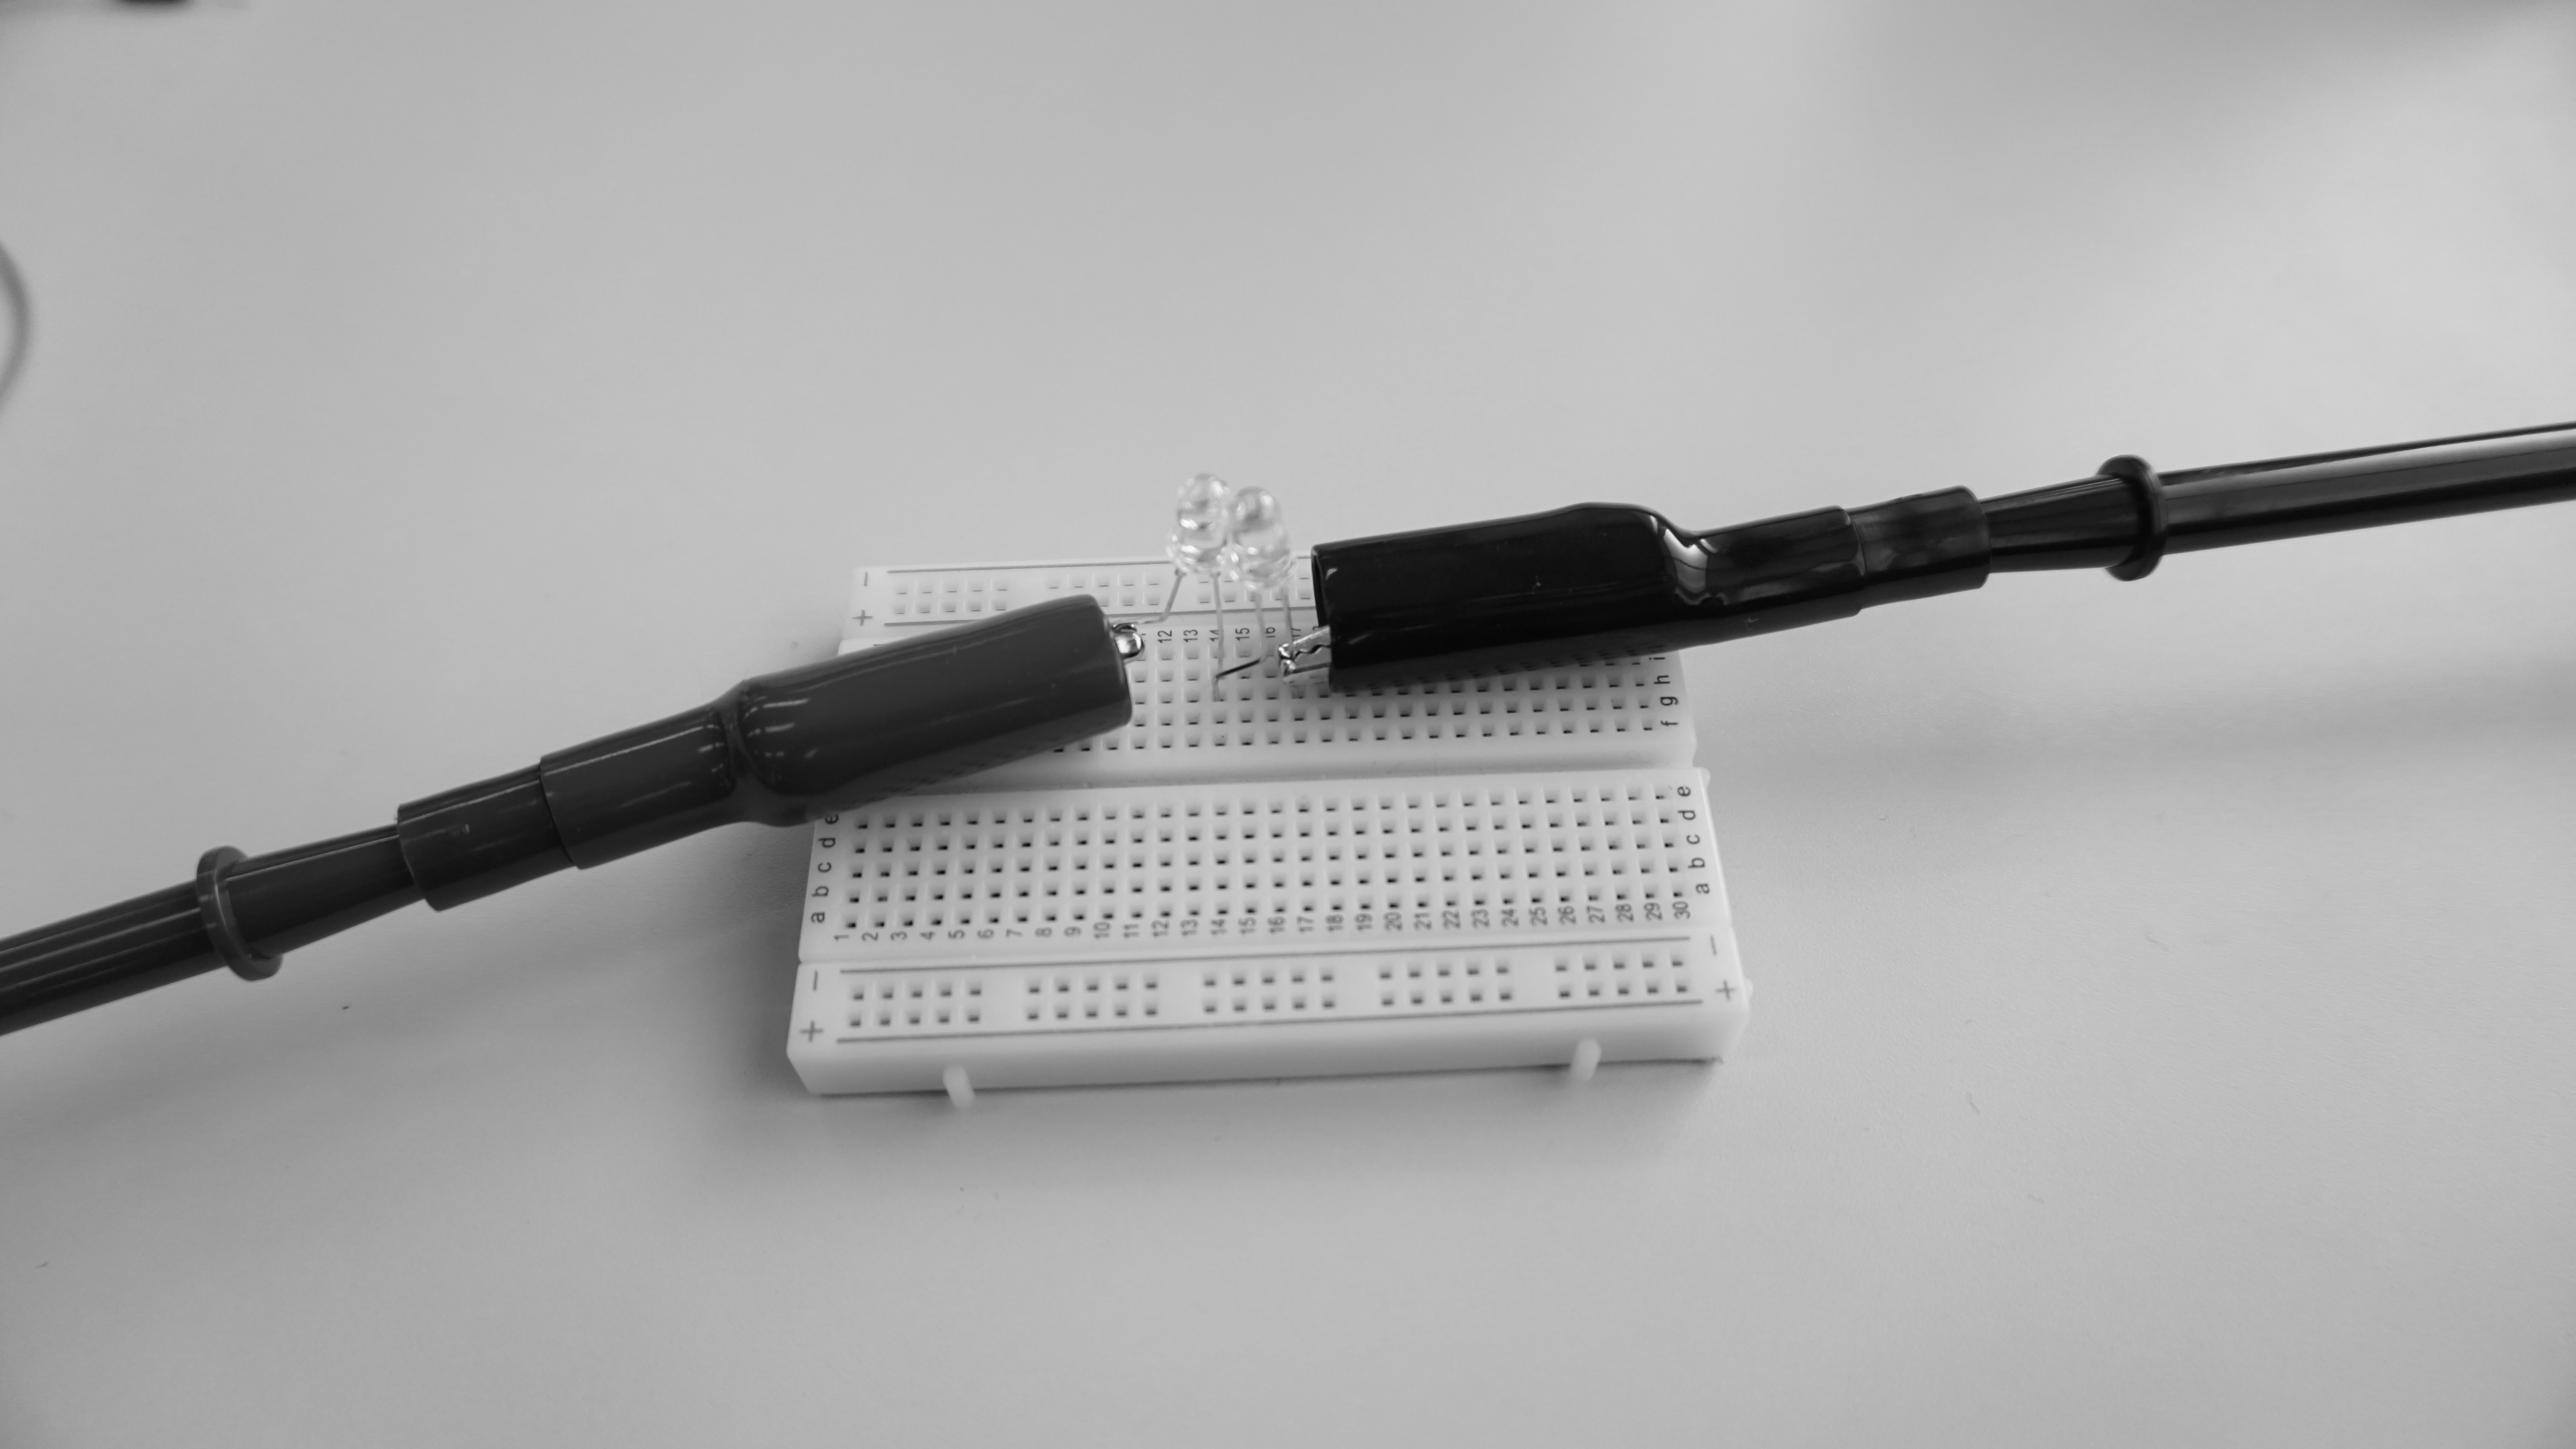
\includegraphics[width=60mm]{./assets/mouse/gray/12.JPG}
    \caption{LED2個で電流と電圧を測定している様子}
    \label{fig:led2}
\end{figure}

次に図\ref{fig:led10}のようにLED10個を直列に接続し、同じくその両端をテスターで見てみました。
その結果、約110$\mu\si\ampere$,約0.5$\si\volt$発生しました。
LED2個の時と比べて電圧が極端に小さくなっていることがわかります。
これはおそらく、LEDの電圧降下の影響をもろに受けてしまったためだと思います。
電流値は、なんかいい感じです。


\begin{figure}[htbp]
    \centering
    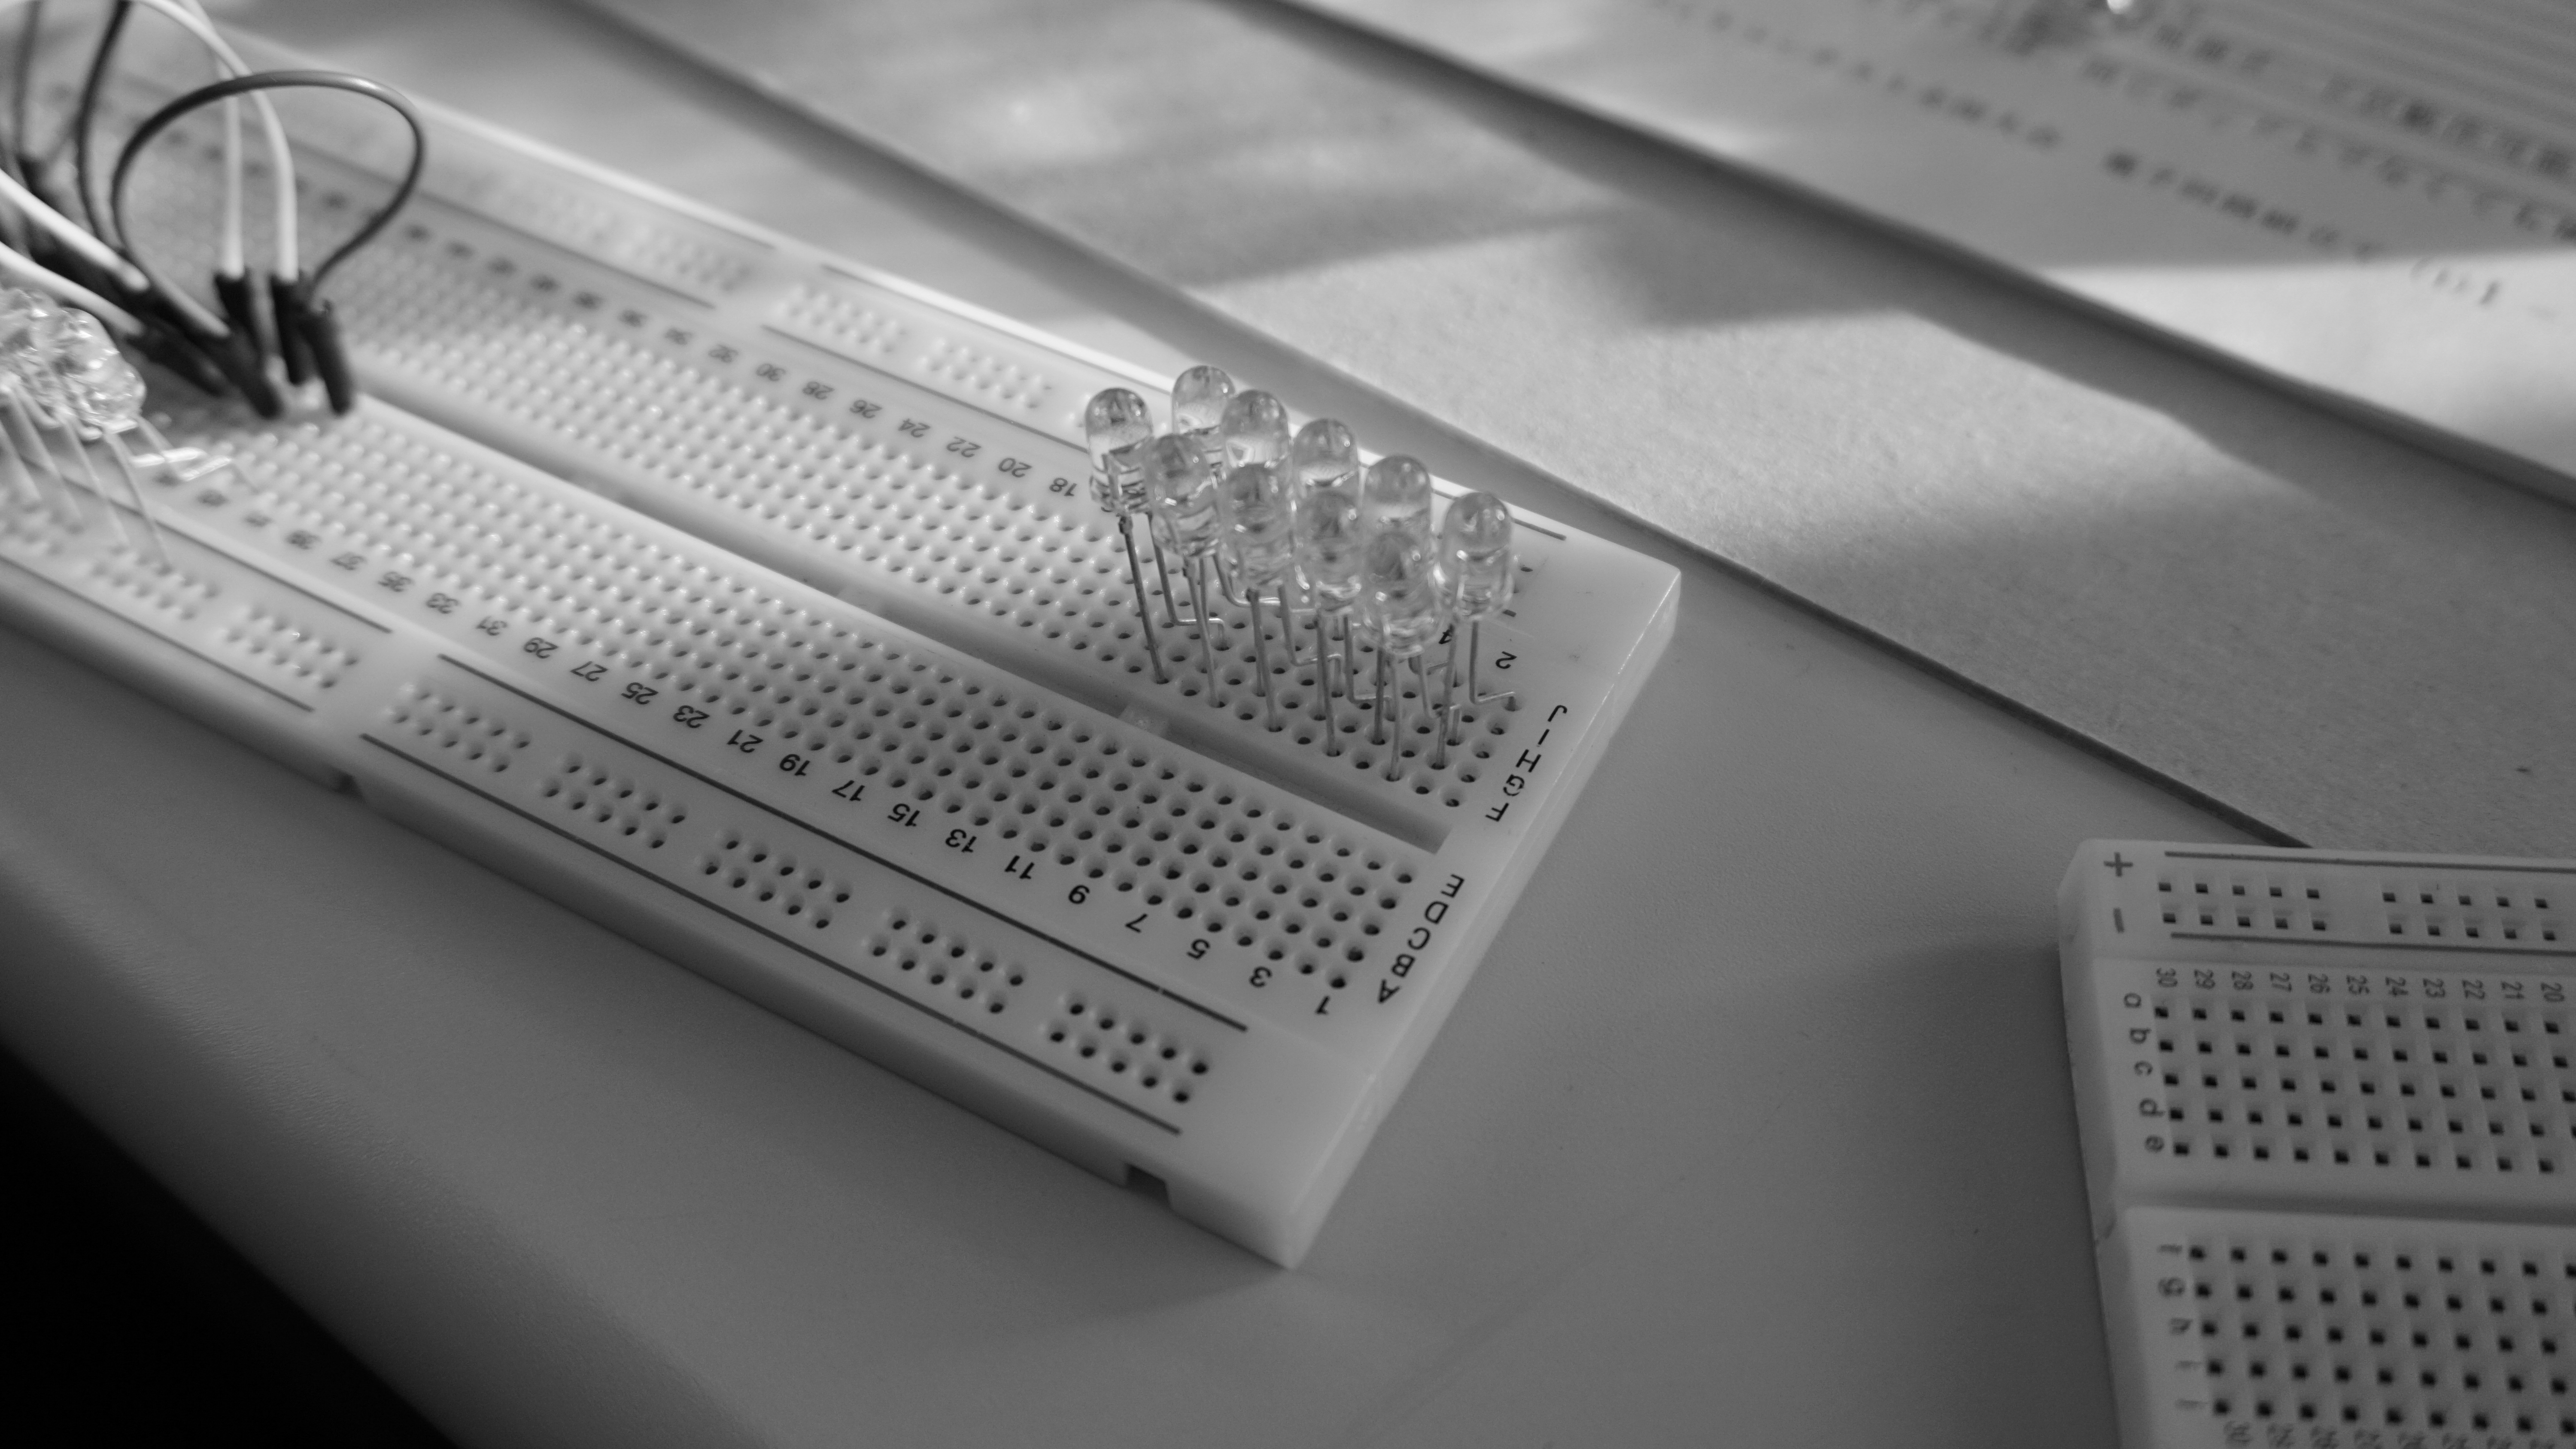
\includegraphics[width=60mm]{./assets/mouse/gray/4.JPG}
    \caption{10個のLEDを接続しているブレッドボード}
    \label{fig:led10}
\end{figure}

図\ref{fig:led_par}のようにLED2個を並列に接続し、同じくテスターで見ていきます。
こちらも太陽光で、同じ時間帯に実験しました。
並列接続の場合、約100$\mu\si\ampere$,1.5$\si\volt$発生しました。


\begin{figure}[htbp]
    \centering
    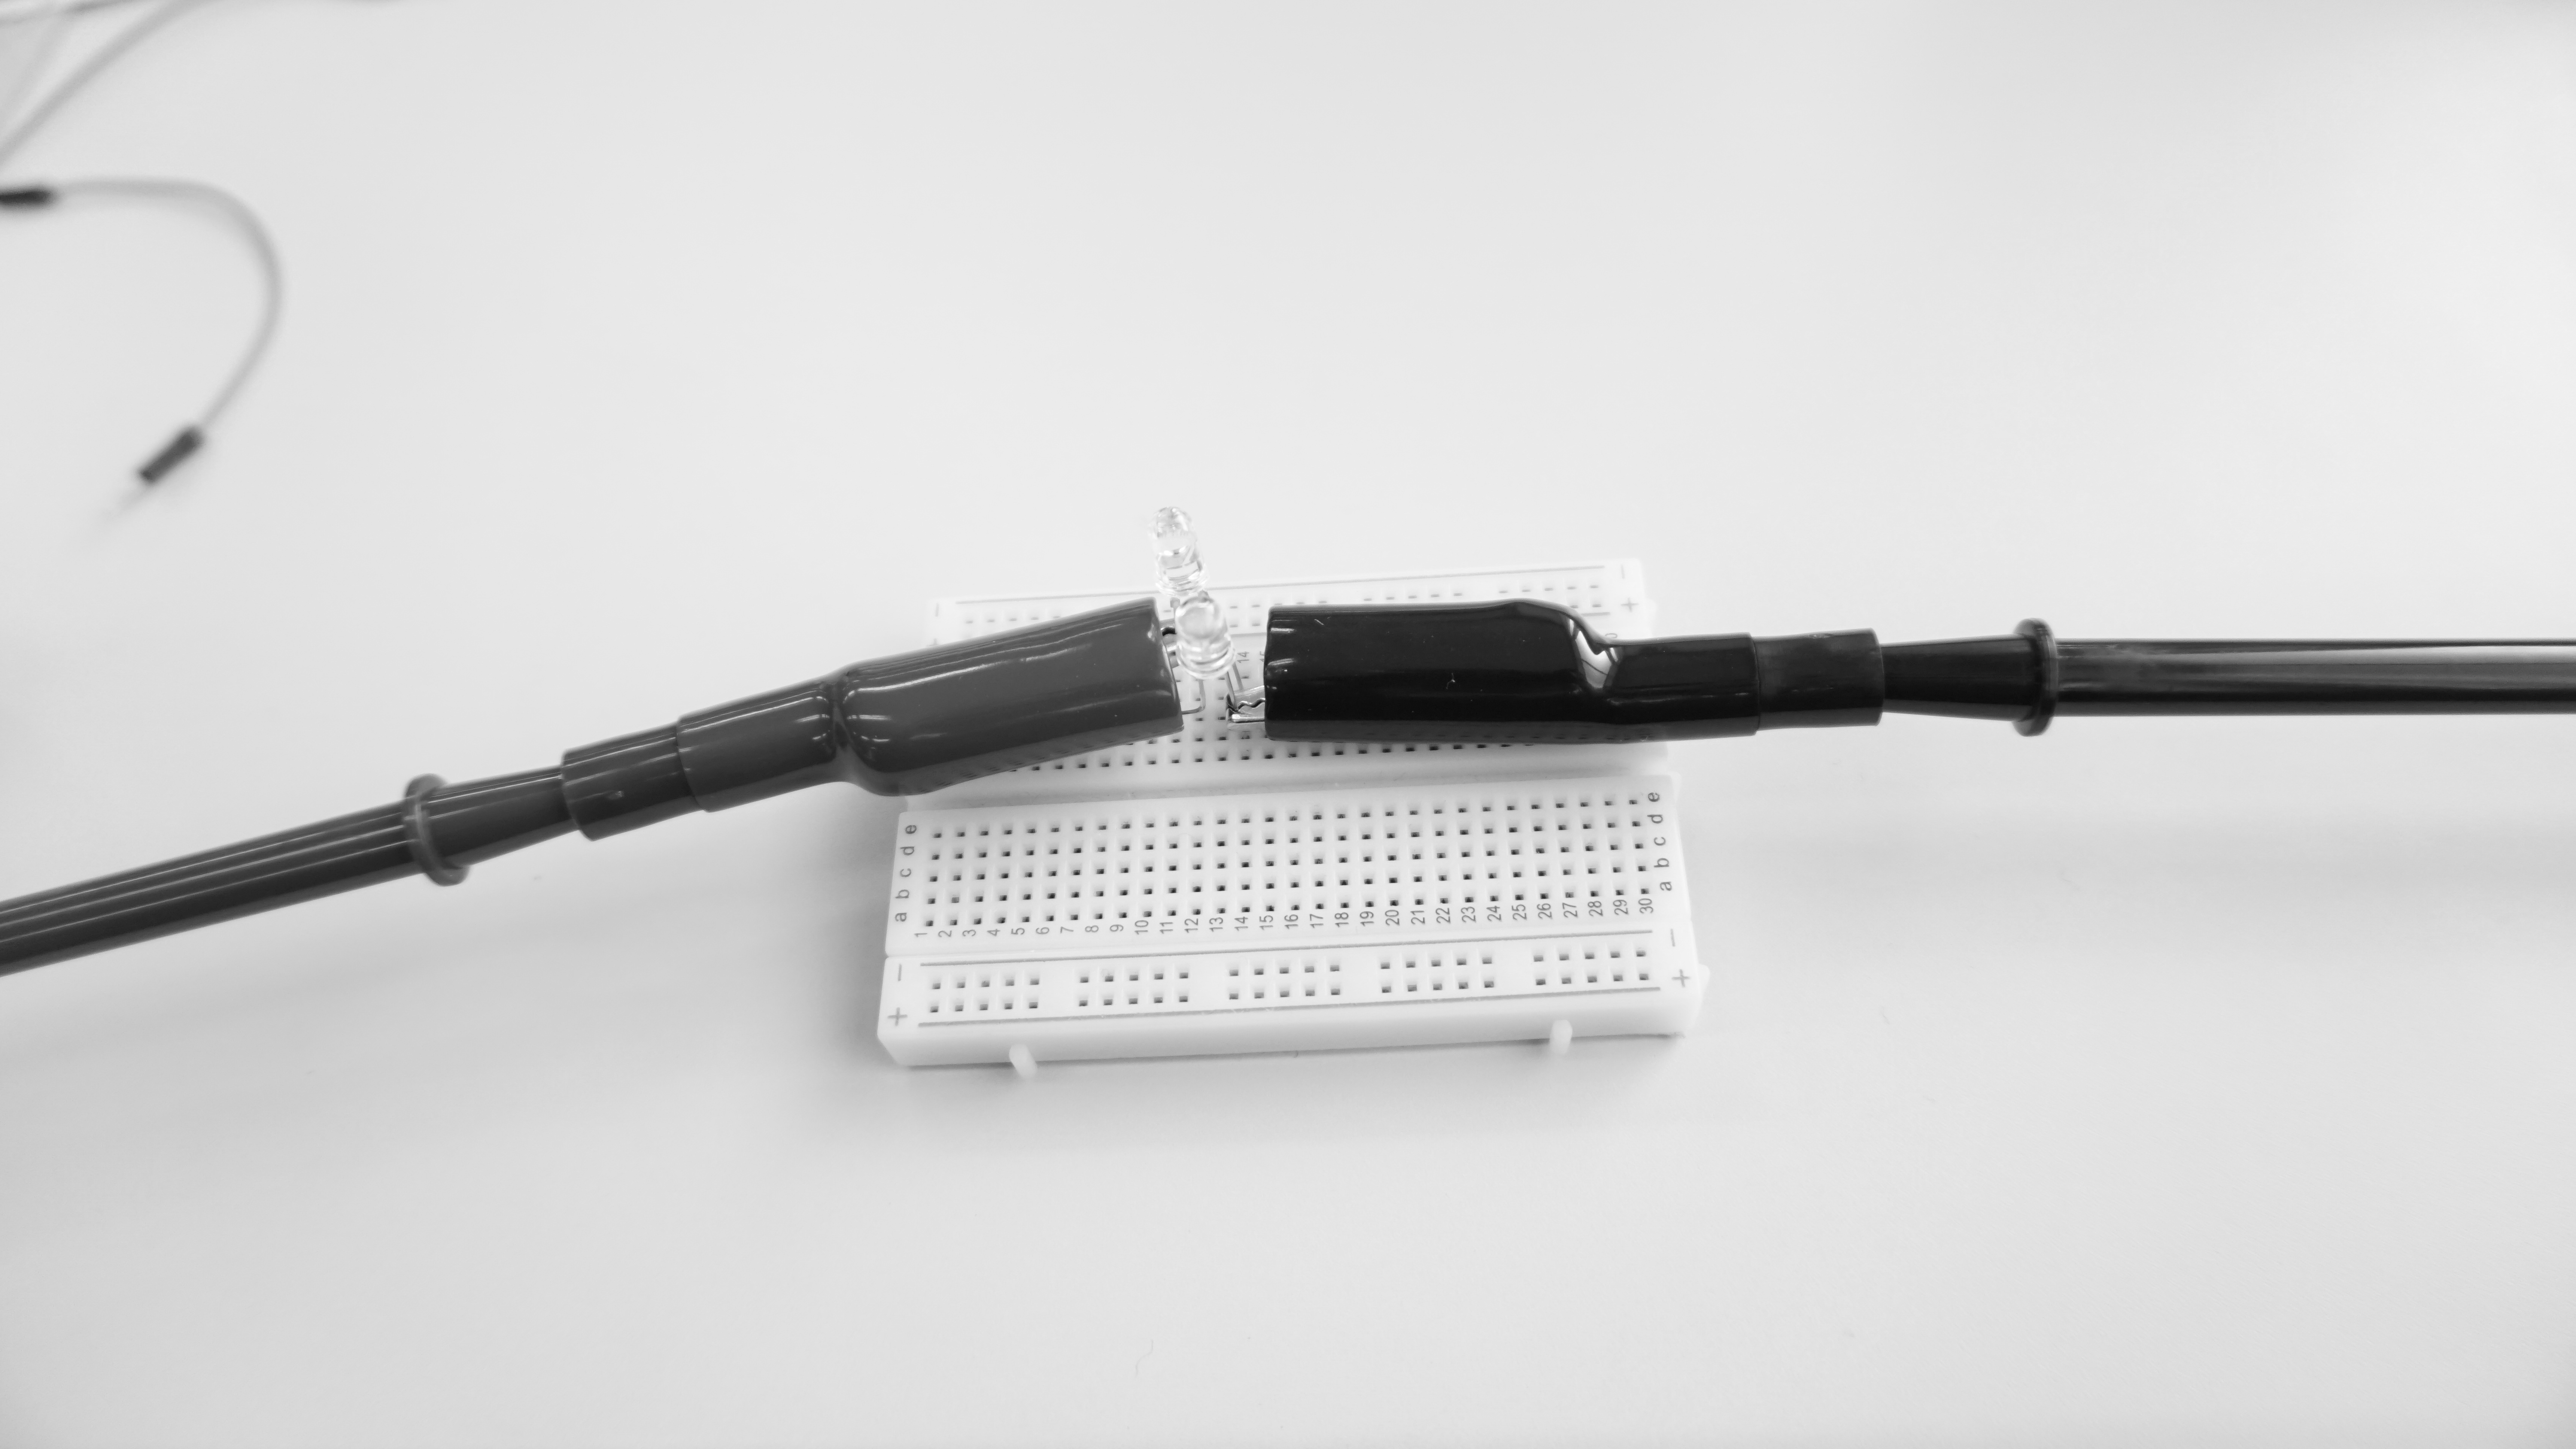
\includegraphics[width=60mm]{./assets/mouse/gray/13.JPG}
    \caption{並列接続したLEDの電流と電圧を測定している様子}
    \label{fig:led_par}
\end{figure}


先ほどと同じく、図\ref{fig:led_par10}のようにLED10個を並列に並べたものの値を取っていきます。
こちらも同じく太陽光で、同じ時間帯です。
この環境で約0.4\si{\milli\ampere},1.5$\si\volt$発生しました。やっと現実味のある数値になってきました。
これは直列と違い抵抗が並列に接続されているためだと思われます。
よくわからないけどいきなり電流が大きくなりました。


\begin{figure}[htbp]
    \centering
    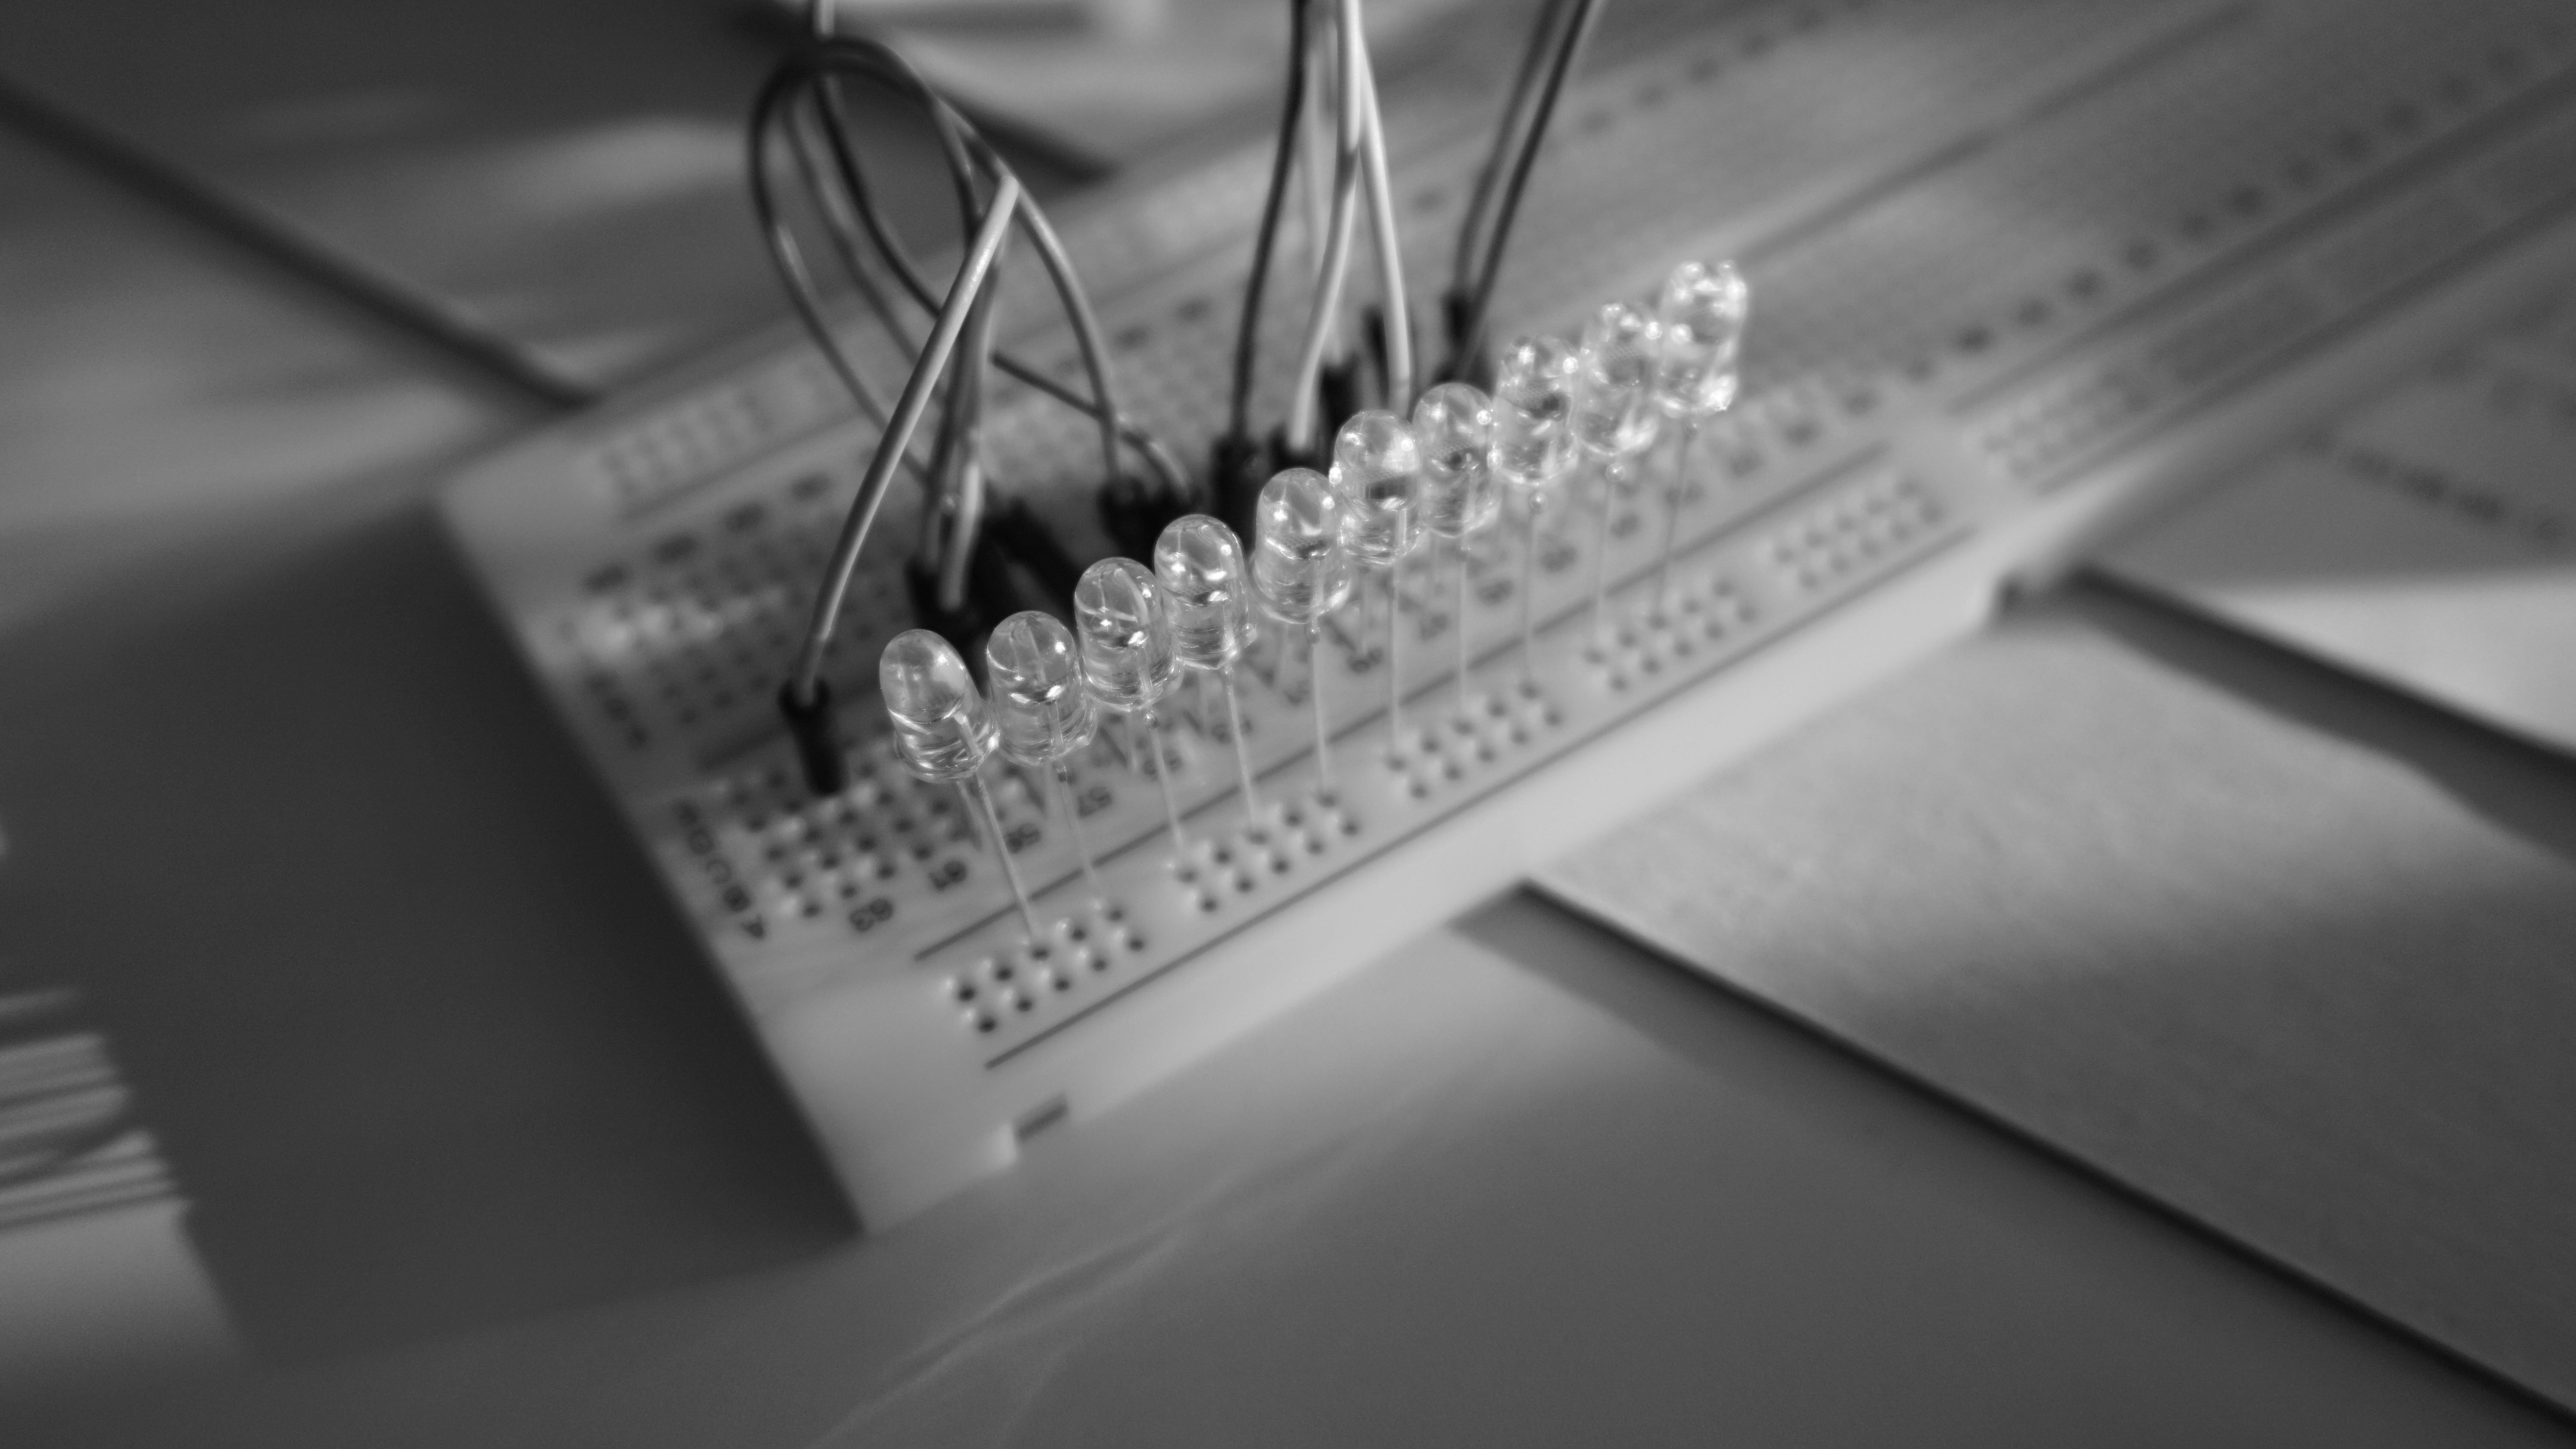
\includegraphics[width=60mm]{./assets/mouse/gray/5.JPG}
    \caption{LED10個を並列接続しているブレッドボード}
    \label{fig:led_par10}
\end{figure}

直流と並列だと並列のほうが優秀だった
並列がなんでこうなったのかはよくわからないです。
とりあえず並列でのほうがLEDを光らせるのには現実的な発電量なので、

\subsection{LEDを30個並べる}

先ほど取れたデータからだと、
LEDを30個並列に並べると1.2\si{\milli\ampere}発生するはずです。
他の実験と同じ日に行いたかったのですが、太陽が沈んでしまったので別の日に実験しました。

\begin{description}
  \item[場所]{ちかくの駐車場}
  \item[時刻]{14:30}
  \item[光源]{太陽光}
  \item[照度]{はかりわすれた}
\end{description}


\begin{figure}[htbp]
    \centering
    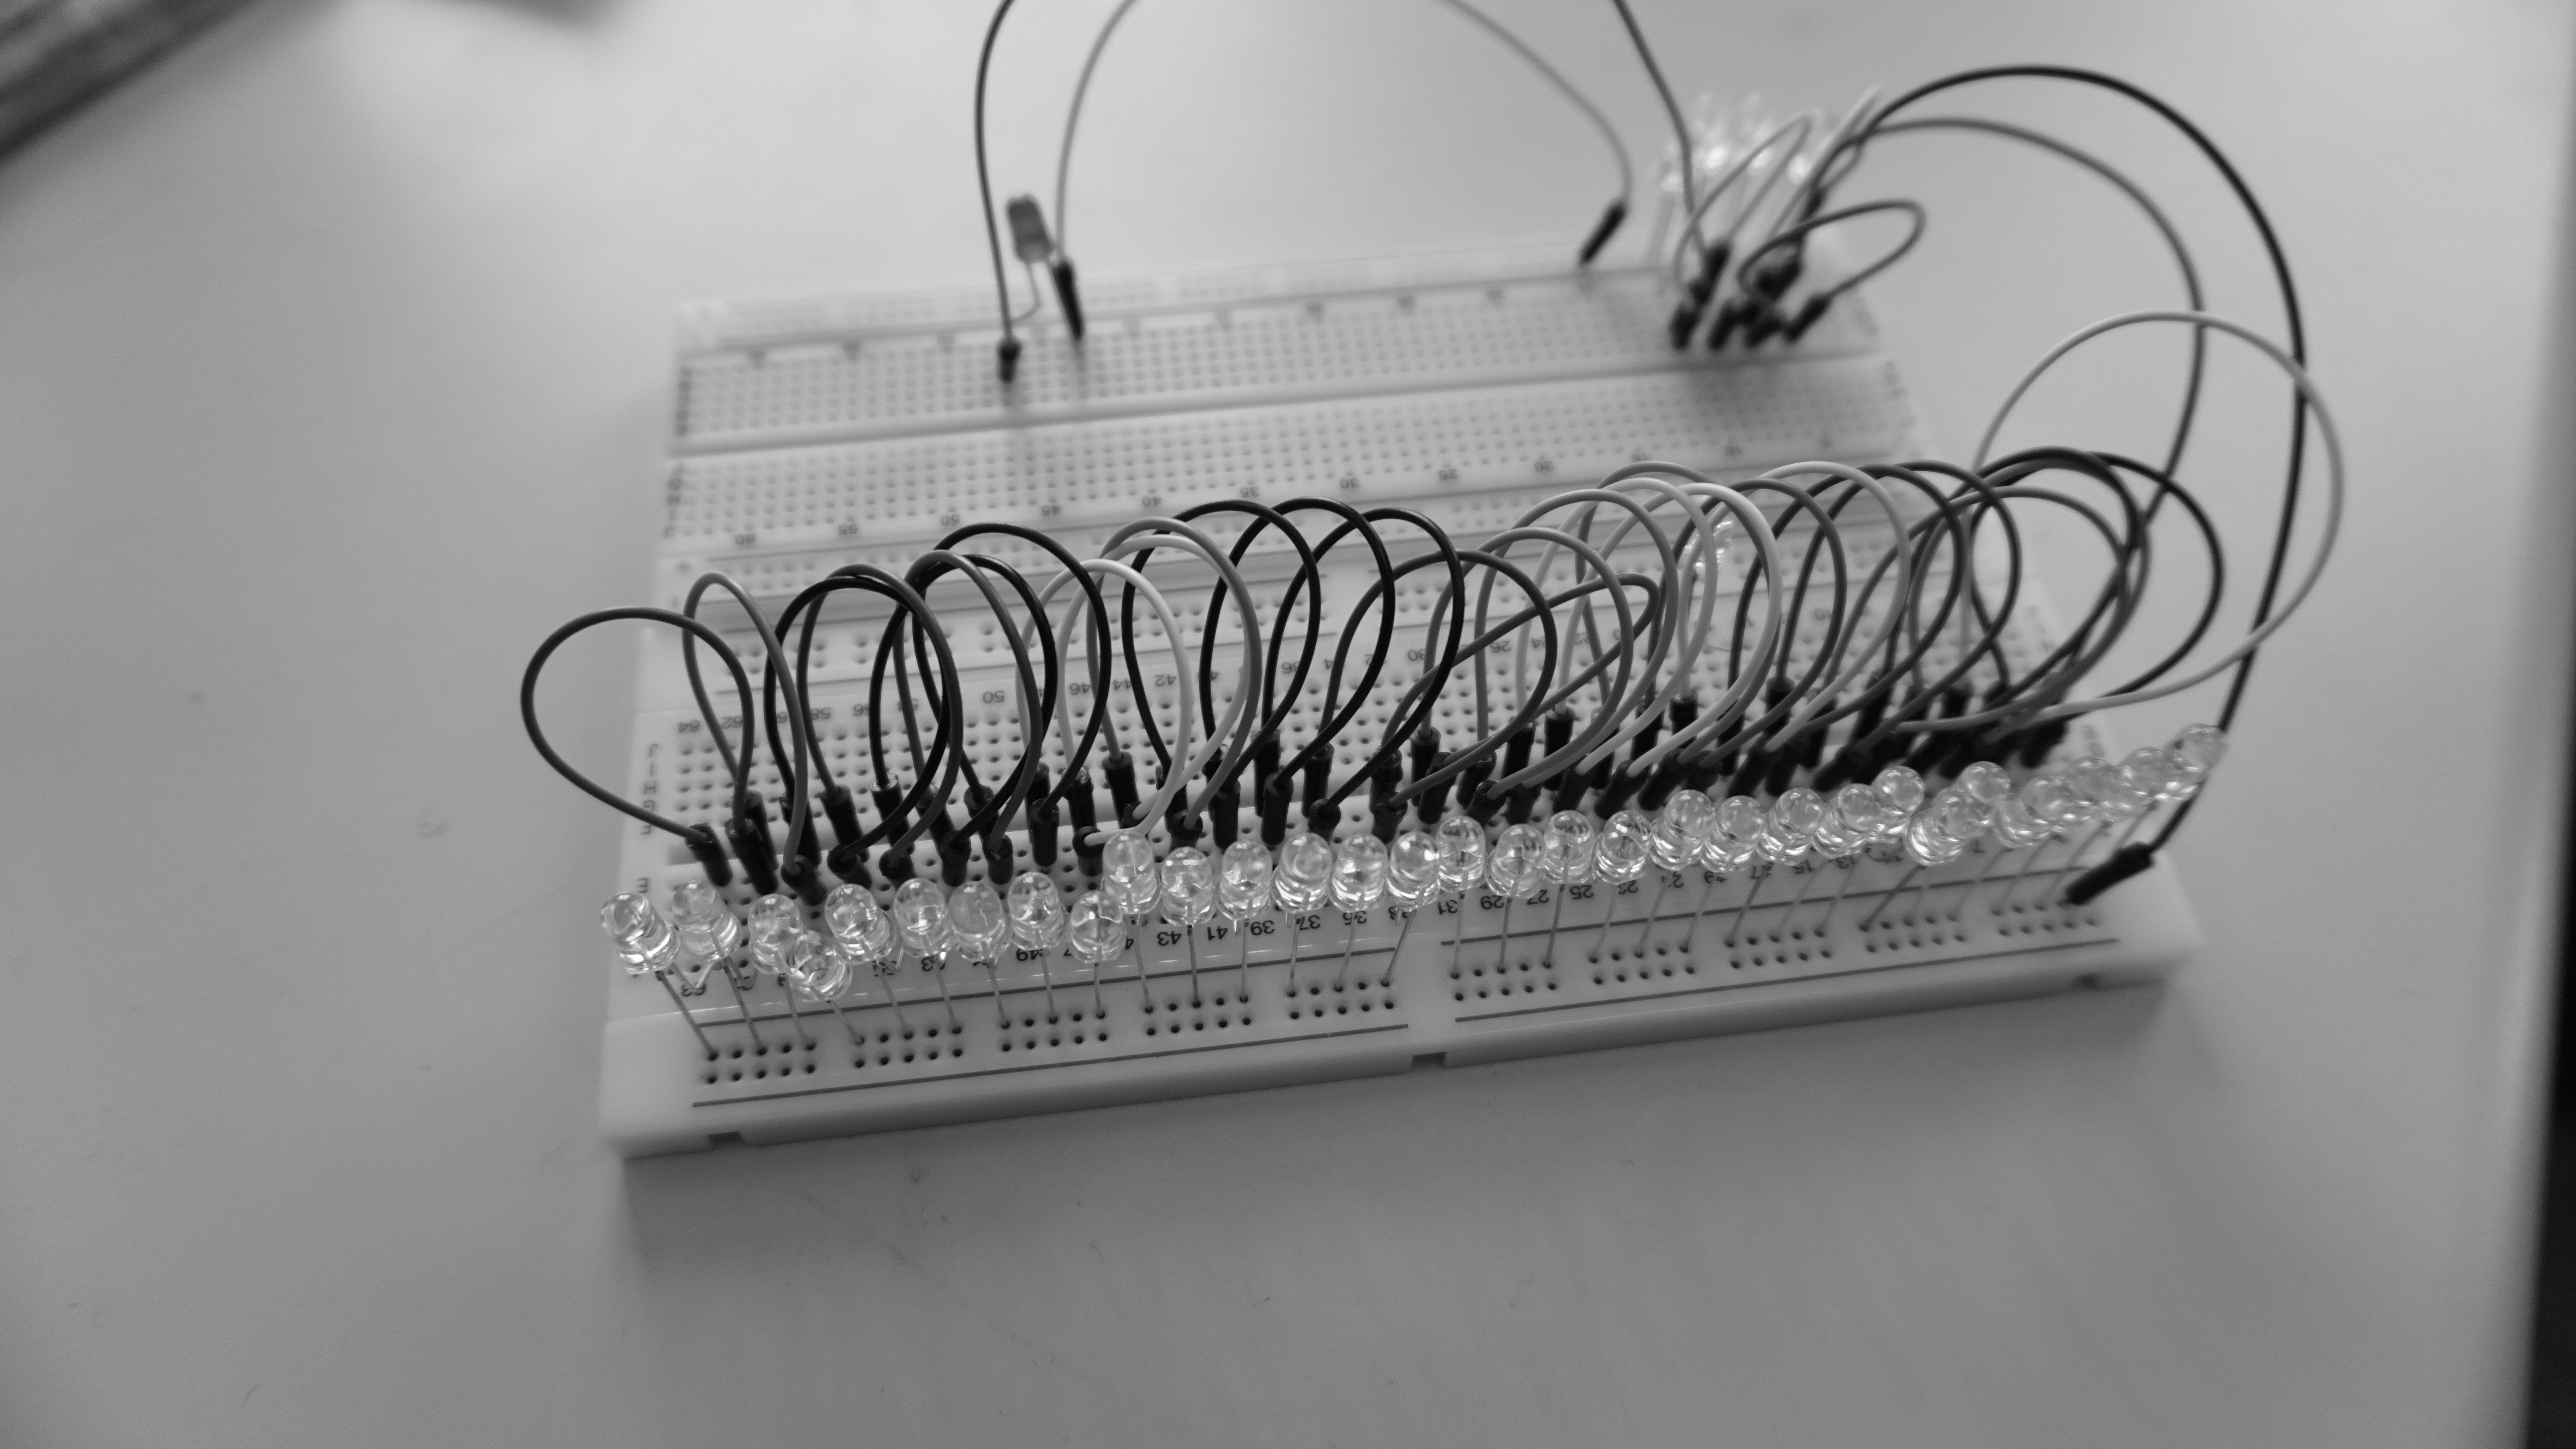
\includegraphics[width=60mm]{./assets/mouse/gray/10.JPG}
    \caption{LEDを30個並べた様子}
    \label{fig:led_par30}
\end{figure}

図\ref{fig:led_par30}のブレッドボードを駐車場へ持って行き太陽の方へLEDを向けました。
このときは、約1\si{\milli\ampere},1.5$\si\volt$となりました。
1\si{\milli\ampere}とはさわると少しぴりぴりするかしないか程度です。また、漏電も1\si{\milli\ampere}以下が許容範囲です。つまり30個並列に並べて発生した電流は漏電にもならないのです。
悲しいですね。

\subsection{波長特性}
LEDにも波長特性はあります。
なので、LEDの色によって発電量も変わってきますし、光源の波長特性によっても全然違います。
場所、光源、LEDをしっかり選ぶとより良い発電ができるかもしれません。
今度検証してみます。

\section{最後に}
LEDで発電するのはあまりお勧めできません。
まともに使おうとしたらたくさん並べなければいけないので、とてもめんどくさいです。
だけど僕はLEDで発電することに喜びを感じているので、これからもLEDで発電していこうとおもいます。


\chapterauthor{ゆひ}
\chapter{後で変える}
\section{自己紹介}
こんにちは,ゆひ(@HSAU\_ dosei)です. 普段はUnityでARアプリ作ってます. 今年も同人誌を書く話になったのでUnityのマスクシェーダーを書いて遊んでみました. 軽めなのでおまけ程度だと思って読んでください.
\section{どんなShader?}
消したいObjectに適用することでそのObjectが消えるShaderです.

\begin{figure}[htbp]
\centering
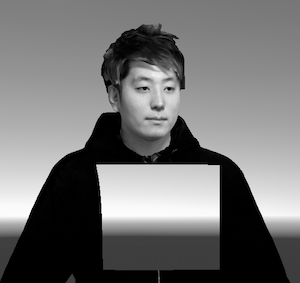
\includegraphics[width=5cm,height=5cm]{./assets/yuhiasset/hsau_dosei2.png}
\end{figure}

白黒で分かりづらいかもしれませんが,こんな感じで重なっている部分が消えて後ろが透けて見えています.

\section{まずShaderを書こう}
Assets/Create/Shader/Standard Surface ShaderからShaderを作成し名前をつけます
今回はStelthとします

\begin{minted}[frame=lines,framesep=2mm,baselinestretch=1.2,fontsize=\footnotesize,linenos,breaklines]{text}
Shader "Custom/Stealth" {
            SubShader {
                Tags { "RenderType"="Opaque" "Queue"="Geometry-1"}
                Pass{

            ColorMask 0

            CGPROGRAM
            #pragma vertex vert
            #pragma fragment frag
            struct appdata{
                float4 vertex : POSITION;
            };
            struct v2f{
                float4 pos : SV_POSITION;
            };
            v2f vert(appdata v){
                v2f o;
                o.pos = UnityObjectToClipPos(v.vertex);
                return o;
            }
            half4 frag (v2f i) : COLOR{
                return half4(0,0,0,0);
            }
            ENDCG
        }
        
    }
}
\end{minted}

一旦中身を消してから中身を記述してあげます!!!
\begin{figure}[htbp]
\centering

\includegraphics[]{./assets/yuhiasset/hsau_dosei1.png}
\caption{Shader}
\label{fig:shader}
\end{figure}
そして作成したShader(図:\ref{fig:shader})を選択し,Create/Material からMaterialを作成します.
Materialの名前は,好きにつけてもらって大丈夫です.

あとはこのMaterialをマスクしたいObjectにつけてあげれば消えます!!

\section{書けたらさっそく使うぞ!!}
さて先程書いてもらったこのShaderですが….
{\bf 何に使えるの?????}
実際このShaderは普通にUnityやっていればあまり使いみちが無いと思います.

しかし、このShaderはARになった途端\bf{化けます}.

\subsection{ex どこでもドア}
\begin{figure}[htbp]
\centering
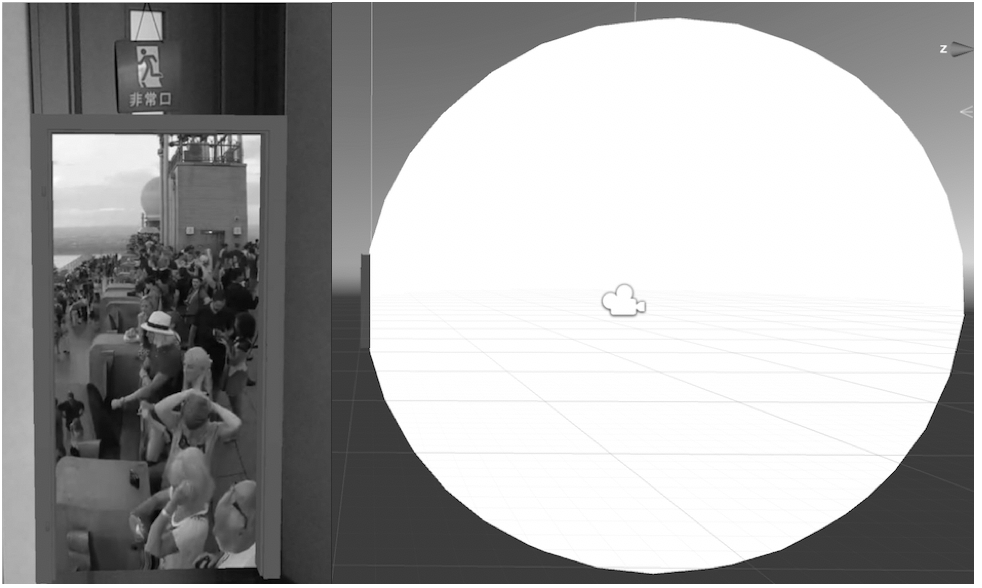
\includegraphics[width=3cm,height=3cm]{./assets/yuhiasset/hsau_dosei3.png}
\end{figure}
この場合、現実世界ではドアのフレームしか見えていませんが,実際には後ろにSphereがあります
当たり前ですが,普通にドアのフレームとSphereを置いただけではドアの後ろにあるSphereが見えてしまいます.そこで先程のShaderをつけたObjrctをドアの周りに配置してマスクすることでドアだけが見えるようになります.
このようにARの場合,ある一定方向から見えてはいけないけど置かないといけないObjectを置かなければならない状況になる場合があります.そういった時にこのShaderはとても{\bf 輝く}のです.

\subsection{ex 空間をマスク}
\begin{figure}[h]
\centering
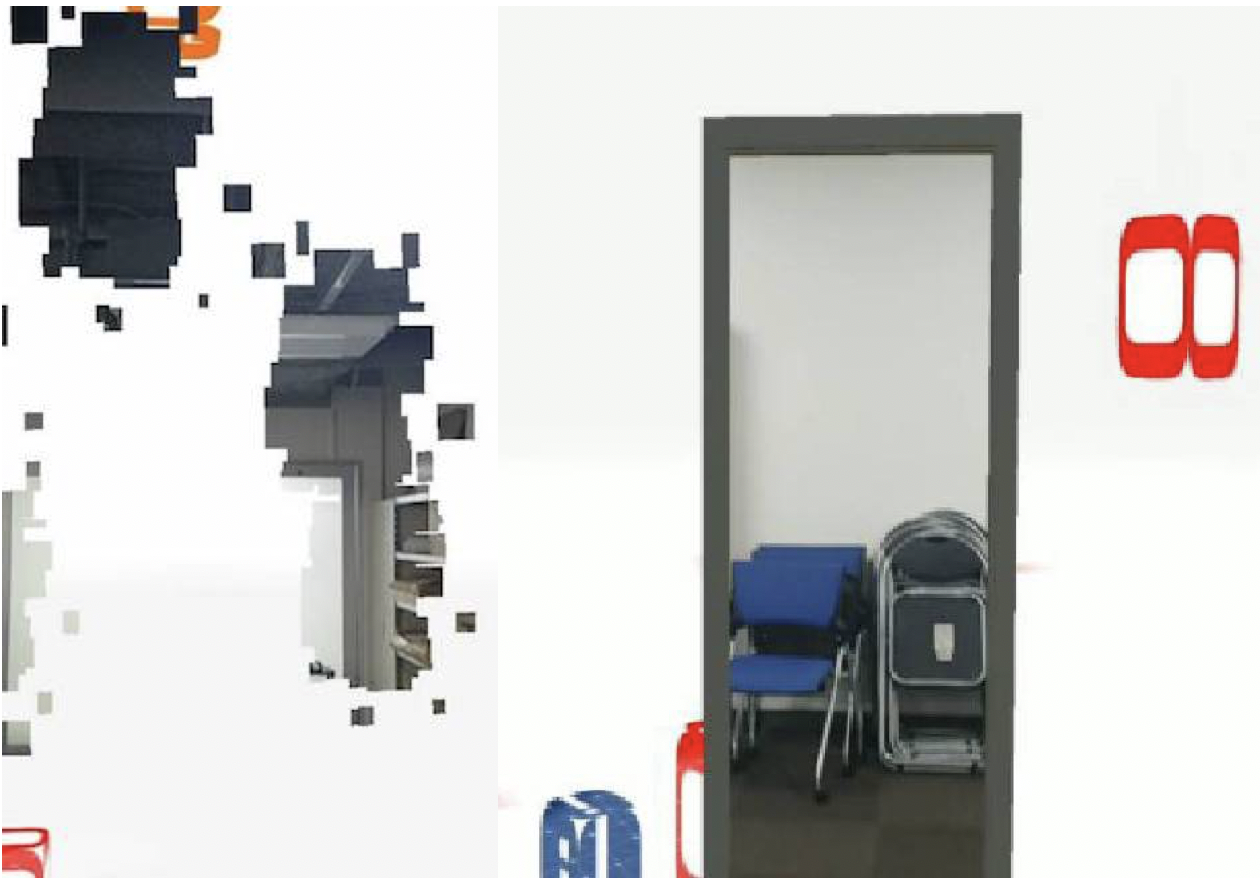
\includegraphics[width=5cm,height=5cm]{./assets/yuhiasset/hsau_dosei6.png}
\end{figure}
この例では外から空間を見るどこでもドアとは対象的にこの例では空間から外を見ています.

通常のARアプリは向こうの世界を覗く,キャラクターがやってくる,といったものが多いと思います.
しかし,その逆をやっているものはほとんどありません.なぜなら空間全てを覆ってしまうとそれはもはや{\bf AR}と呼べなくなってしまうから.{\bf AR}の良い所は現実の空間を{\bf 拡張}することで普段ありえないような体験ができることだと僕は考えます,程よく現実世界を露出させてあげるとすごく{\bf エモく
なります.
そこでこのShaderでマスクすることで現実世界が露出し{\bf エモさ}が増すのです.

\section{最後に}
結局Shaderの話ではなくARの話になってしまいましたが,きっとマスクシェーダーを用いることでできるようになる表現について分かってもらえたと\sout{勝手}に思っています。
今回はARでの使用例について取り上げましたが,他にもまだまだ使いみちがあるはずです!

{\bf 組み合わせは無限大!君の想像次第で無限に使えるぞ!}

ゆひ


\chapterauthor{すとんりばー}
\chapter{後で変える}
\section{はじめに}



\newpage
\myimpression[%
name=LOCAL Students\\情報ボーイズの寄稿ノート, %
author=うっひょい, \and %
ちくうぇいと, \and %
あわあわ, \\ \and %
けんつ, \and %
さわだ, \and %
Jumpaku, \and %
あるねこ, %
date=2018年4月22日, %
publisher=LOCAL学生部, %
print=有限会社ねこのしっぽ %
]%
\end{document}
